% Options for packages loaded elsewhere
\PassOptionsToPackage{unicode}{hyperref}
\PassOptionsToPackage{hyphens}{url}
%
\documentclass[
]{article}
\usepackage{amsmath,amssymb}
\usepackage{iftex}
\ifPDFTeX
  \usepackage[T1]{fontenc}
  \usepackage[utf8]{inputenc}
  \usepackage{textcomp} % provide euro and other symbols
\else % if luatex or xetex
  \usepackage{unicode-math} % this also loads fontspec
  \defaultfontfeatures{Scale=MatchLowercase}
  \defaultfontfeatures[\rmfamily]{Ligatures=TeX,Scale=1}
\fi
\usepackage{lmodern}
\ifPDFTeX\else
  % xetex/luatex font selection
    \setmainfont[Numbers=Lowercase,Numbers=Proportional]{Skolar PE}
    \setsansfont[]{Skolar Sans PE}
\fi
% Use upquote if available, for straight quotes in verbatim environments
\IfFileExists{upquote.sty}{\usepackage{upquote}}{}
\IfFileExists{microtype.sty}{% use microtype if available
  \usepackage[]{microtype}
  \UseMicrotypeSet[protrusion]{basicmath} % disable protrusion for tt fonts
}{}
\makeatletter
\@ifundefined{KOMAClassName}{% if non-KOMA class
  \IfFileExists{parskip.sty}{%
    \usepackage{parskip}
  }{% else
    \setlength{\parindent}{0pt}
    \setlength{\parskip}{6pt plus 2pt minus 1pt}}
}{% if KOMA class
  \KOMAoptions{parskip=half}}
\makeatother
\usepackage{xcolor}
\usepackage[top=20mm,left=25mm,right=25mm,bottom=20mm]{geometry}
\usepackage{longtable,booktabs,array}
\usepackage{calc} % for calculating minipage widths
% Correct order of tables after \paragraph or \subparagraph
\usepackage{etoolbox}
\makeatletter
\patchcmd\longtable{\par}{\if@noskipsec\mbox{}\fi\par}{}{}
\makeatother
% Allow footnotes in longtable head/foot
\IfFileExists{footnotehyper.sty}{\usepackage{footnotehyper}}{\usepackage{footnote}}
\makesavenoteenv{longtable}
\usepackage{graphicx}
\makeatletter
\def\maxwidth{\ifdim\Gin@nat@width>\linewidth\linewidth\else\Gin@nat@width\fi}
\def\maxheight{\ifdim\Gin@nat@height>\textheight\textheight\else\Gin@nat@height\fi}
\makeatother
% Scale images if necessary, so that they will not overflow the page
% margins by default, and it is still possible to overwrite the defaults
% using explicit options in \includegraphics[width, height, ...]{}
\setkeys{Gin}{width=\maxwidth,height=\maxheight,keepaspectratio}
% Set default figure placement to htbp
\makeatletter
\def\fps@figure{htbp}
\makeatother
\setlength{\emergencystretch}{3em} % prevent overfull lines
\providecommand{\tightlist}{%
  \setlength{\itemsep}{0pt}\setlength{\parskip}{0pt}}
\setcounter{secnumdepth}{-\maxdimen} % remove section numbering
% definitions for citeproc citations
\NewDocumentCommand\citeproctext{}{}
\NewDocumentCommand\citeproc{mm}{%
  \begingroup\def\citeproctext{#2}\cite{#1}\endgroup}
\makeatletter
 % allow citations to break across lines
 \let\@cite@ofmt\@firstofone
 % avoid brackets around text for \cite:
 \def\@biblabel#1{}
 \def\@cite#1#2{{#1\if@tempswa , #2\fi}}
\makeatother
\newlength{\cslhangindent}
\setlength{\cslhangindent}{1.5em}
\newlength{\csllabelwidth}
\setlength{\csllabelwidth}{3em}
\newenvironment{CSLReferences}[2] % #1 hanging-indent, #2 entry-spacing
 {\begin{list}{}{%
  \setlength{\itemindent}{0pt}
  \setlength{\leftmargin}{0pt}
  \setlength{\parsep}{0pt}
  % turn on hanging indent if param 1 is 1
  \ifodd #1
   \setlength{\leftmargin}{\cslhangindent}
   \setlength{\itemindent}{-1\cslhangindent}
  \fi
  % set entry spacing
  \setlength{\itemsep}{#2\baselineskip}}}
 {\end{list}}
\usepackage{calc}
\newcommand{\CSLBlock}[1]{\hfill\break\parbox[t]{\linewidth}{\strut\ignorespaces#1\strut}}
\newcommand{\CSLLeftMargin}[1]{\parbox[t]{\csllabelwidth}{\strut#1\strut}}
\newcommand{\CSLRightInline}[1]{\parbox[t]{\linewidth - \csllabelwidth}{\strut#1\strut}}
\newcommand{\CSLIndent}[1]{\hspace{\cslhangindent}#1}
\usepackage{indentfirst}
\setlength\parindent{24pt}
\usepackage[left]{lineno}
\modulolinenumbers[1]
\usepackage{multicol}
\usepackage{setspace}
\usepackage{float}
\usepackage{afterpage}
\usepackage{stfloats}
\usepackage{graphicx}
\newcommand{\hideFromPandoc}[1]{#1}
 \let\Begin\begin \let\End\end
\usepackage[labelfont=bf]{caption}
\captionsetup{labelfont=bf}
\usepackage{amsmath}
\DeclareMathOperator\arctanh{arctanh}
\makeatletter
\@ifpackageloaded{subfig}{}{\usepackage{subfig}}
\@ifpackageloaded{caption}{}{\usepackage{caption}}
\captionsetup[subfloat]{margin=0.5em}
\AtBeginDocument{%
\renewcommand*\figurename{Fig}
\renewcommand*\tablename{Table}
}
\AtBeginDocument{%
\renewcommand*\listfigurename{List of Figures}
\renewcommand*\listtablename{List of Tables}
}
\newcounter{pandoccrossref@subfigures@footnote@counter}
\newenvironment{pandoccrossrefsubfigures}{%
\setcounter{pandoccrossref@subfigures@footnote@counter}{0}
\begin{figure}\centering%
\gdef\global@pandoccrossref@subfigures@footnotes{}%
\DeclareRobustCommand{\footnote}[1]{\footnotemark%
\stepcounter{pandoccrossref@subfigures@footnote@counter}%
\ifx\global@pandoccrossref@subfigures@footnotes\empty%
\gdef\global@pandoccrossref@subfigures@footnotes{{##1}}%
\else%
\g@addto@macro\global@pandoccrossref@subfigures@footnotes{, {##1}}%
\fi}}%
{\end{figure}%
\addtocounter{footnote}{-\value{pandoccrossref@subfigures@footnote@counter}}
\@for\f:=\global@pandoccrossref@subfigures@footnotes\do{\stepcounter{footnote}\footnotetext{\f}}%
\gdef\global@pandoccrossref@subfigures@footnotes{}}
\@ifpackageloaded{float}{}{\usepackage{float}}
\floatstyle{ruled}
\@ifundefined{c@chapter}{\newfloat{codelisting}{h}{lop}}{\newfloat{codelisting}{h}{lop}[chapter]}
\floatname{codelisting}{Listing}
\newcommand*\listoflistings{\listof{codelisting}{List of Listings}}
\makeatother
\ifLuaTeX
  \usepackage{selnolig}  % disable illegal ligatures
\fi
\usepackage{bookmark}
\IfFileExists{xurl.sty}{\usepackage{xurl}}{} % add URL line breaks if available
\urlstyle{same}
\hypersetup{
  pdftitle={Reassessing the modularity of gene co-expression networks using the Stochastic Block Model},
  pdfauthor={Diogo Melo1,2,, Luisa F. Pallares1,2,3, and Julien F. Ayroles1,2,},
  pdfkeywords={modularity, gene
co-expression, WGCNA, MMC, clustering, RNA-seq, GO enrichment},
  hidelinks,
  pdfcreator={LaTeX via pandoc}}

\title{Reassessing the modularity of gene co-expression networks using
the Stochastic Block Model}
\author{Diogo Melo\textsuperscript{1,2,*},
Luisa F. Pallares\textsuperscript{1,2,3}, and
Julien F. Ayroles\textsuperscript{1,2,*}}
\date{}

\newfontfamily\titlefont{Skolar Sans PE}

\usepackage{titlesec}
\newfontfamily\sectionfont{Skolar Sans PE}
\titleformat*{\section}{\Large\bfseries\sectionfont}
\titleformat*{\subsection}{\large\bfseries\sectionfont}
\titleformat*{\subsubsection}{\normalsize\bfseries\sectionfont}

\begin{document}
\makeatletter
\renewcommand{\maketitle}{\setlength{\parindent}{0pt}
\begin{flushleft}
    \huge{\titlefont \textbf{Reassessing the modularity of gene
co-expression networks using the Stochastic Block Model}}
    
          \vspace{0.2cm}
      \small{Manuscript v2.1 - \today}
    
    \vspace{0.2cm}

    \Large{Diogo Melo\textsuperscript{1,2,*},
Luisa F. Pallares\textsuperscript{1,2,3}, and
Julien F. Ayroles\textsuperscript{1,2,*}}

    \vspace{0.3cm}

\end{flushleft}
}
\makeatother
\maketitle



\footnotesize
\textsuperscript{1} Lewis-Sigler Institute for Integrative Genomics,
Princeton University, Princeton, NJ, USA\\
\textsuperscript{2} Department of Ecology and Evolutionary Biology,
Princeton University, Princeton, NJ, USA\\
\textsuperscript{3} Friedrich Miescher Laboratory of the Max Planck
Society, Tübingen, Germany

\href{mailto:damelo@princeton.edu}{*damelo@princeton.edu (DM)};
\href{mailto:jayroles@princeton.edu}{*jayroles@princeton.edu (JA)}

\normalsize

\section{Abstract}\label{abstract}

Finding communities in gene co-expression networks is a common first
step toward extracting biological insight from these complex datasets.
Most community detection algorithms expect genes to be organized into
assortative modules, that is, groups of genes that are more associated
with each other than with genes in other groups. While it is reasonable
to expect that these modules exist, using methods that assume they exist
a priori is risky, as it guarantees that alternative organizations of
gene interactions will be ignored. Here, we ask: can we find meaningful
communities without imposing a modular organization on gene
co-expression networks, and how modular are these communities? For this,
we use a recently developed community detection method, the weighted
degree corrected stochastic block model (SBM), that does not assume that
assortative modules exist. Instead, the SBM attempts to efficiently use
all information contained in the co-expression network to separate the
genes into hierarchically organized blocks of genes. Using RNA-seq gene
expression data measured in two tissues derived from an outbred
population of \textit{Drosophila melanogaster}, we show that (a) the SBM
is able to find ten times as many groups as competing methods, that (b)
several of those gene groups are not modular, and that (c) the
functional enrichment for non-modular groups is as strong as for modular
communities. These results show that the transcriptome is structured in
more complex ways than traditionally thought and that we should revisit
the long-standing assumption that modularity is the main driver of the
structuring of gene co-expression networks.

\section{Author Summary}\label{author-summary}

Understanding how genes work together is crucial for unraveling the
biological processes underlying complex traits. To gain insight into
these genetic interactions, researchers often analyze gene co-expression
networks, in which genes are linked based on the similarity of their
expression patterns among different individuals. Traditionally, it has
been assumed that these networks are organized into distinct assortative
modules, in which genes are more connected to each other within modules
than between them. However, by using a novel non-parametric clustering
approach called the Stochastic Block Model, we show that fruit fly
transcriptomes contain not only assortative, modular gene clusters, but
also functionally relevant non-modular clusters that would be overlooked
by standard methods. This suggests that transcriptional networks may be
more complex and diverse than previously thought. Our findings highlight
the importance of using unbiased clustering techniques to fully capture
the various architectures of gene co-expression networks and their
potential biological significance.

\newpage

\section{Introduction}\label{introduction}

\linenumbers
\doublespacing

Gene co-expression networks inform our understanding of cell and
organismal function by encoding associations between genes. Associations
between expression levels can indicate common function, and the number
of connections can point to central or regulatory genes
{[}\citeproc{ref-Van_Dam2018-nf}{1}{]}. Due to the large dimensionality
of gene expression data, often composed of several thousands of gene
expression measures, a major tool in the analysis of co-expression is
gene clustering: separating the genes into related groups, which can
then be explored separately {[}\citeproc{ref-Dhaeseleer2005-jv}{2}{]}.
This drastically reduces the number of genes we need to consider at the
same time and allows for the identification of hubs or centrally
connected genes that can be used to inform further experimental
validation
{[}\citeproc{ref-Langfelder2008-qa}{3},\citeproc{ref-Imenez_Silva2017-ic}{4}{]}.

The question is, given a co-expression network, how should we cluster
the genes? The general idea behind several methods is to look for
similar genes, as these are expected to be involved in related
biological functions. However, several definitions of similarity have
been used. The most basic measure of similarity borrows from classical
morphological integration theory and attempts to find gene modules based
on their correlations. In this context, genes in the same module are
expected to be highly correlated and perform similar functions, while
genes in different modules are expected to have low correlations
{[}\citeproc{ref-Olson1958-fh}{5}--\citeproc{ref-Wagner2007-jt}{7}{]}.
Here, we refer to this classic pattern of higher within- than
between-group correlation as assortativity, and to the groups as
assortative modules. Other methods use the correlations to create other
measures of similarity, which are then used as input to clustering
algorithms. Weighted gene co-expression network analysis {[}WGCNA,
\citeproc{ref-Langfelder2008-qa}{3}{]} uses a power transformation of
the correlation between gene expressions (or a topological similarity
measure built with these transformed correlations)
{[}\citeproc{ref-Zhang2005-kh}{8},\citeproc{ref-Dong2007-ff}{9}{]} as a
similarity measure that is then separated into assortative modules using
hierarchical clustering. One of the main objectives of WGCNA is finding
hub genes, which have high connectivity within modules and are clearly
identified by hierarchical clustering. Other methods borrow from network
analysis and attempt to explicitly maximize the Newman Modularity
{[}\citeproc{ref-Newman2006-fv}{10}{]} of the weighted gene network. For
example, Modulated Modularity Clustering {[}MMC,
\citeproc{ref-Stone2009-hv}{11}{]} uses an adaptive algorithm to find a
non-linear distance between genes based on their correlations that
maximizes the number of modules uncovered by maximizing modularity.
Although these methods differ in their definition of similarity, they
all impose an assortative structure on the gene expression network, in
which similar genes are expected to be more correlated with each other
than with other genes.

Clustering genes in tightly correlated modules aligns with the intuition
that groups of genes performing similar functions should be highly
correlated. However, imposing assortativity will necessarily ignore
alternative organizations, if they exist, and could prevent us from
fully understanding of how transcriptional networks are organized. For
example, Betzel et al. {[}\citeproc{ref-Betzel2018-ec}{12}{]} provides
several examples of network organization besides assortativity, like
non-assortative networks, in which vertices have more edges to vertices
between communities than within; or core-periphery, in which a central
community is connected to other communities, but the peripheral
communities are not internally connected
(Fig~\ref{fig:network_structure}). These alternative architectures can
also occur in the same network simultaneously
{[}\citeproc{ref-Betzel2018-ec}{12},\citeproc{ref-Peel2018-ai}{13}{]}.
We currently lack the empirical information on how common these patterns
are in gene co-expression data, simply because our widely applied
methods are completely blind to them due to their exclusive focus on
assortativity. Given that other biological networks, like neuronal
networks
{[}\citeproc{ref-Betzel2018-ec}{12},\citeproc{ref-Peixoto2018-or}{14}{]},
exhibit clear evidence for these alternative organizations, there is no
reason to think that a system as complex and as high-dimensional as the
transcriptome should be limited to a single pattern of organization. To
explicitly address this possibility of alternative organizations, we use
a more general measure of similarity that allows us to find meaningful
gene groups that are not necessarily assortative but still have clear
biological interpretation. This approach is implemented in the weighted
nested Degree Corrected Stochastic Block Model
{[}\citeproc{ref-Peixoto2018-or}{14},wnDC-SBM, or SBM for brevity,
\citeproc{ref-Peixoto2017-zw}{15}{]}, which has shown promising results
in similar applications
{[}\citeproc{ref-Baum2019-ty}{16},\citeproc{ref-Morelli2021-ge}{17}{]}.
The SBM is different from other clustering methods in that it does not
attempt to find assortative modules (i.e., modules with higher within-
than between-module correlation). Instead, any information contained in
the gene co-expression network can potentially be used to inform the
clustering. Genes can be clustered together because they share similar
patterns of connectivity to other genes, regardless of whether they are
more strongly correlated with each other or with genes in other
clusters. The word \emph{information} here should be understood in the
information theoretical sense: in the SBM, clusters are inferred so as
to minimize the number of bits required to represent the network given
the information about the clusters
{[}\citeproc{ref-Peixoto2023-xd}{18}{]}. To be sure, the SBM can capture
an assortative modular pattern if it is present, but it is general
enough to also capture other network organizations
{[}\citeproc{ref-Betzel2018-ec}{12},\citeproc{ref-Zhang2020-up}{19}{]}.
Furthermore, even if, in the context of the SBM, assortativity is not
the main driver of gene partitioning, it can still be used to interpret
the clusters we obtain. By measuring the modularity of the identified
clusters, we can compare networks with respect to their modularity
without the problem of comparing a measure that was maximized to find
the clusters in the first place. This opens the possibility of an
unbiased comparison of the degree of modularity in different
transcriptional networks (e.g., different cell types, tissues, species,
etc.), which is a question that remains unexplored so far.

\begin{figure}
\centering
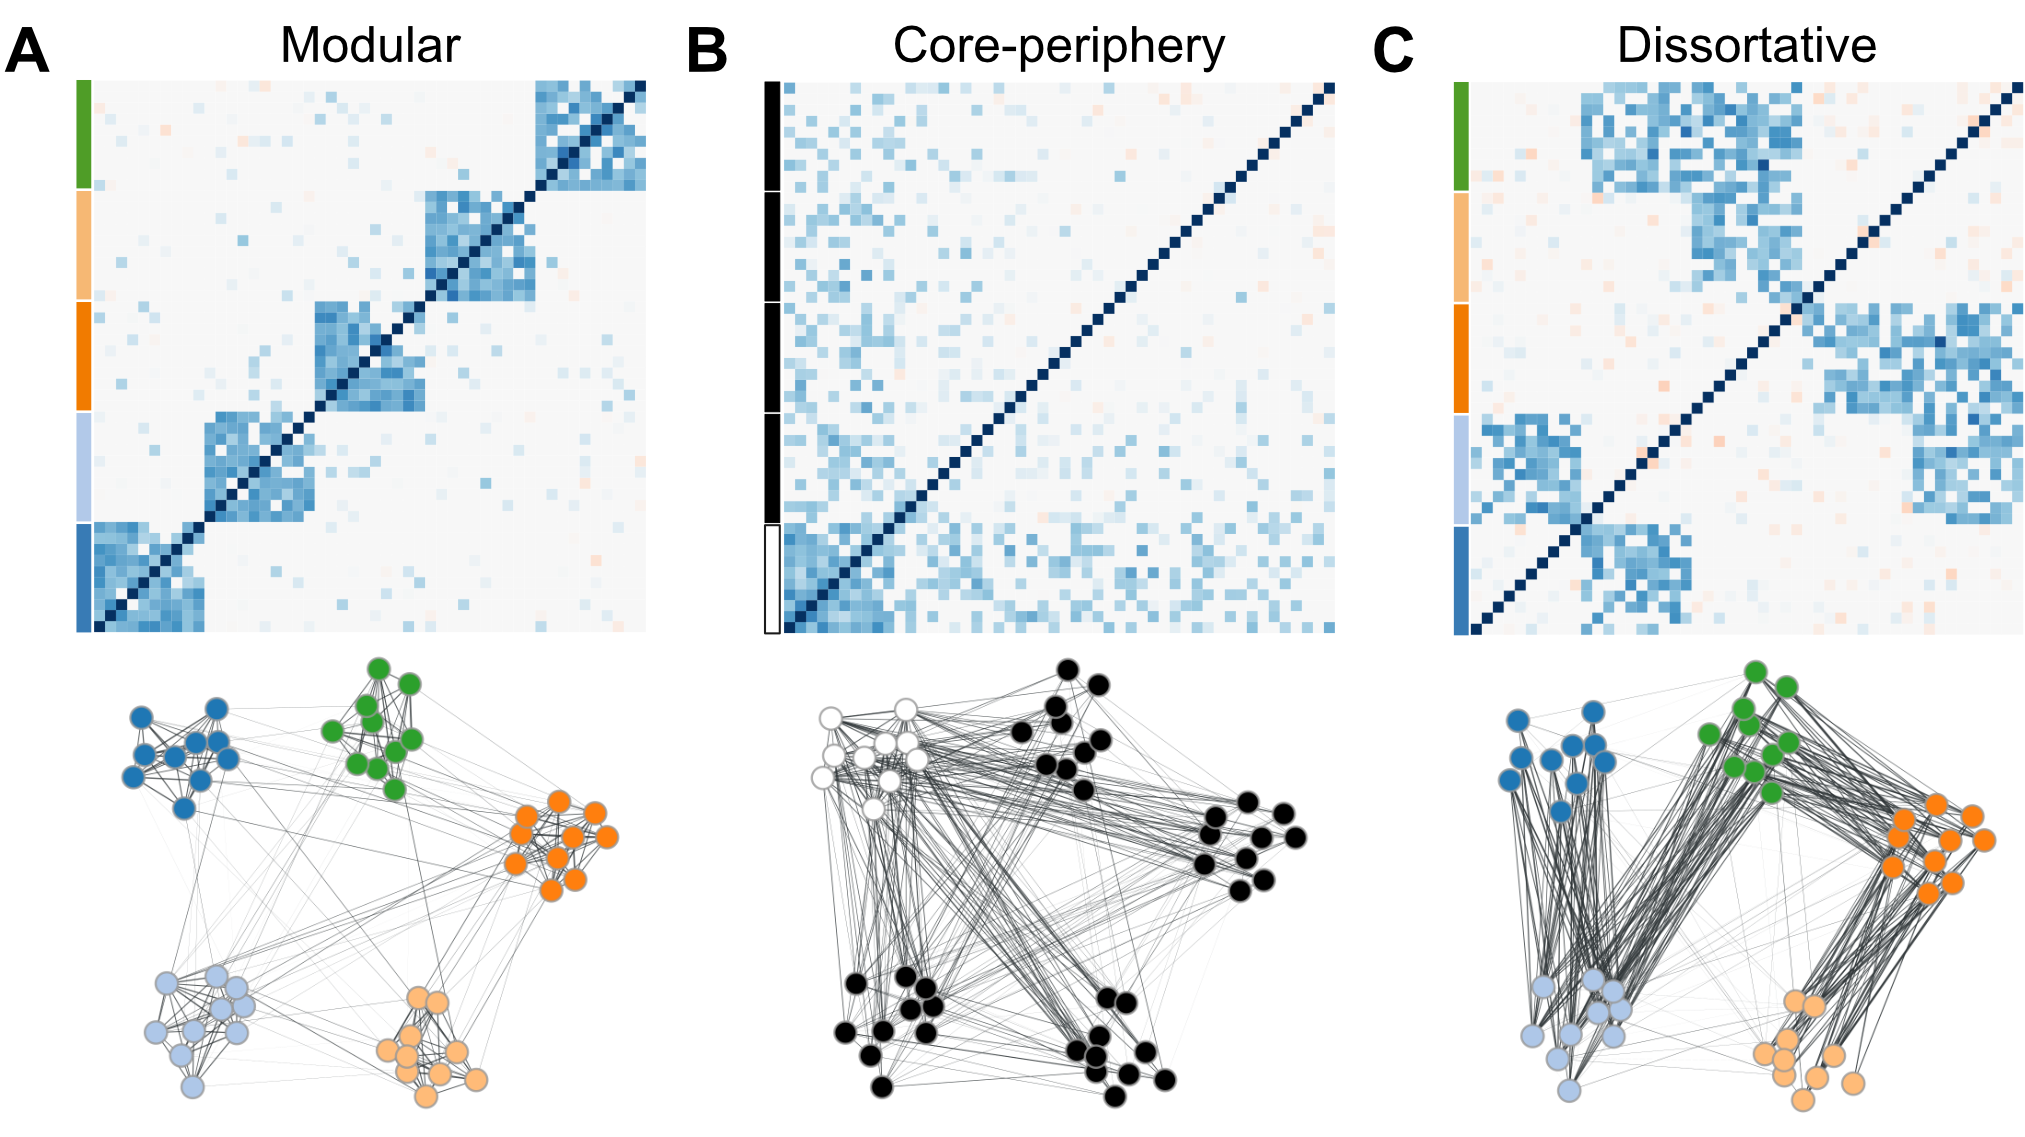
\includegraphics[width=\textwidth,height=9cm]{figures/network_strucuture_figure.png}
\caption{Schematic representation of three network architectures. Each
panel shows the adjacency matrix (top) and the corresponding network
diagram (bottom). (A) Modular architecture: The network is composed of
five distinct modules, each containing ten interconnected traits.
Modules are connected by a few inter-module links. (B) Core-periphery
architecture: The network consists of a single densely connected core
module with ten traits and a peripheral group with 40 traits. Peripheral
group is connected to the core module, but has few internal connections.
(C) Disassortative architecture: The network comprises five groups, each
with ten traits. Traits within each group are not interconnected but are
instead connected to traits in other groups, forming a pattern of
between-group connections.}\label{fig:network_structure}
\end{figure}

Here, using a multi-tissue RNAseq dataset from \emph{Drosophila
melanogaster}, we show first, that the SBM, a model with no free
parameters, can find many more gene clusters than competing methods.
Second, that such gene clusters are biologically meaningful, as revealed
by highly specific gene ontology enrichment. Third, that biological
meaning is not restricted to assortative modules as traditionally
thought but extends to the non-assortative parts of the transcriptome.
Our results highlight the importance of using clustering algorithms that
don't rely on assortativity metrics to explore the structure of
transcriptomes in a comprehensive and unbiased manner.

\section{Methods}\label{methods}

\subsection{Gene expression measures}\label{gene-expression-measures}

Elsewhere {[}\citeproc{ref-Pallares2023-eQTL}{20}{]}, we quantified
whole-genome gene expression in hundreds of outbred \emph{Drosophila
melanogaster} female flies using a high-throughput RNAseq library
preparation protocol {[}TM3seq, \citeproc{ref-Pallares2020-ha}{21}{]}.
To build the gene co-expression networks, here we use a subset of the
full dataset that includes: samples for two tissues, head (n = 212) and
body (n = 252), individuals with the best coverage (average gene counts:
head = 4.65M, body = 4.58M), and genes with moderate to high expression
(average CPM \textgreater{} 5 and detected in every sample, head n =
5584 genes, body n = 5533 genes). The expression matrices used to
generate co-expression networks correspond to VOOM-transformed gene
counts (SI Data 1) {[}\citeproc{ref-Law2014-xl}{22}{]} where the effect
of known and unknown {[}\citeproc{ref-Leek2007-bx}{23}{]} covariates was
removed using the function removeBatchEffect from the R package limma
{[}\citeproc{ref-Law2014-xl}{22}{]}. Details on the collection of RNAseq
data, library preparation, and processing of raw RNAseq counts can be
found in {[}\citeproc{ref-Pallares2023-eQTL}{20}{]}.

\subsection{Gene co-expression
network}\label{gene-co-expression-network}

Using the gene expression measures for both tissues, we generate
co-expression network graphs. In theory, we could proceed using a full
network in which all pairs of genes are connected but fitting the SBM
with this fully connected graph is computationally too onerous.
Moreover, given the very large number of correlations being estimated,
many of these estimates are likely to be spurious or noisy. To mitigate
these issues, we reduce the connectivity of the network by imposing a
stringent Benjamini-Hochberg (BH) false discovery rate (FDR) cut-off on
the edges. This approach removes edges with a large p-value associated
with the correlation between the corresponding genes, thus retaining
only the most statistically significant correlations that we are more
confident reflect true biological relationships. As edges are removed,
some genes with only non-significant correlations become disconnected
from the rest of the network and can be removed. By gradually reducing
the FDR threshold, we reduce the density of the gene network while
attempting to keep as many genes as possible, until we arrive at a
viable network with which to fit the SBM. We chose an FDR such that we
reduce the graph density as much as possible (targeting a density of
around 5\%, corresponding to about 500,000 edges in the graphs) while
still retaining most genes. Using this heuristic, we arrive at an FDR of
1\% for the head and 0.1\% for the body datasets which kept most of the
genes (94.2\% in the head:5261, and 92.6\% in the body:5124) while
reducing the graph density to a manageable level for use in the SBM,
allowing the SBM to be fit in under a week of computational time. This
same set of genes is used to compare two clustering methods: WGCNA and
SBM. This choice of FDR is arbitrary but represents a pragmatic
trade-off between computational feasibility, network sparsity, and
retention of biologically relevant information. The chosen thresholds
aim to strike a balance between these competing factors and provide a
reasonable starting point for the application of the SBM to these large
gene co-expression networks. Alternative thresholds could have been
chosen, potentially leading to different downstream results, and to
assess the effects of the FDR choice, we performed a sequence of SBM
fits with a random subset of around 200 genes, showing that the main
results should be robust to wide range of FDR choices (SI Fig 1).

\subsection{Edge weights}\label{edge-weights}

Each method uses different edge weights for the network graph. WGCNA can
use the fully connected graph, so we maintain all edges in these
methods. We use the topological overlap matrix (TOM) similarity in
WGCNA. We use the low-density graph described above for the SBM, with
the edge weight given by twice the inverse hyperbolic tangent
transformed Spearman correlations between gene expressions. This
transformation allows the edge weights to be modeled by normal
distributions in the SBM, as we discuss below.

\subsection{Stochastic Block Model}\label{stochastic-block-model}

The Weighted Nested Degree Corrected Stochastic Block Model
{[}\citeproc{ref-Karrer2011-vp}{24}{]} is a Bayesian generative model
that attempts to find the partition with the highest posterior
probability given the observed network and edge weights. Broadly
speaking, this is achieved by dividing the network into groups of genes,
called blocks, and modeling the weight and existence of a link between
two genes in a network solely on their belonging to a particular block.
So, genes with similar patterns of connections tend to be clustered in
the same block. The degree correction refers to a modification of the
standard Stochastic Block Model that allows genes with different degrees
to be clustered in the same block {[}see
\citeproc{ref-Peixoto2017-zw}{15} for details{]}.

If \(b\) is a particular partition of the genes in the weighted gene
network \(A\), we write a model that generates \(A\) with probability
given by \(P(A| b, \theta)\), where \(\theta\) stands in for any extra
parameter we need besides the group partition \(b\). With this model, we
can write the posterior probability of the block partition \(b\) given
the observed network:

\[
P(b|A) = \frac{P(A|\theta, b)P(\theta, b)}{P(A)}
\]

where \(P(A)\) is a normalization constant. In the canonical form of the
Stochastic Block Model, the parameters \(\theta\) are related to the
expected number of edges between and within blocks. Specifically, the
model would include parameters related to the expected number of edges
between blocks \(r\) and \(s\), and parameters representing the expected
degree of nodes in block \(r\). These parameters are used to generate
edges independently according to a Poisson distribution, meaning that
the actual number of edges between blocks and the degrees of nodes can
vary from the expected values. However, here, we use the microcanonical
formulation from {[}\citeproc{ref-Peixoto2018-or}{14}{]}. The
microcanonical formulation of the Stochastic Block Model does not have
any free parameters \(\theta\). Instead, it imposes hard constraints on
the network structure, requiring that the networks that are given
non-null probabilities by \(P(A| b)\) have exactly the same number of
edges between blocks and the same degree sequence as the observed
network. In this formulation, the total number of edges between blocks
\(r\) and \(s\) is fixed to the observed value \(e_{rs}\), and the
degree of each node is also fixed to its observed value \(k_i\). This
means that the microcanonical SBM generates networks with exactly the
same block-wise edge counts and degree sequence as the observed network.
Furthermore, the microcanonical formulation allows for the exact
calculation of the probability of a network given a partition, which is
useful for model selection and hypothesis testing. The probability of a
network given a partition under the microcanonical assumption is simply
the number of ways of observing that network divided by all possible
networks that respect the constraints imposed by the block structure and
the degree sequence. The mathematical expression for this probability is
not particularly illuminating, so we refer the reader to
{[}\citeproc{ref-Peixoto2017-zw}{15}{]} for the gory details. To provide
some intuition about the idea behind this model, we can think about how,
given the community labels, we can represent the network in a compact
way using only the total number of edges (and their weights, see below)
between and within each block. The inference task is therefore to find
the partition \(b\) that has maximal probability given the observation
of the measured network, which is determined by the the constraints
imposed by the edges, weights, and degree sequence.

\subsubsection{Description length}\label{description-length}

We can also describe this inference of the optimal partition in the
context of information theory. The posterior probability of the block
partition can be written as:

\[
P(b|A) \propto \exp(-\Sigma)
\]

Where \(\Sigma = -\log[P(A|\theta, b)] - \log[P(\theta,b)]\) is called
the description length of the gene network \(A\), and has an
information-theoretic interpretation, being the amount of information
required to encode the network given \(\theta\) and \(b\). So, finding
the partition with maximal posterior probability is the same as
minimizing the description length, or, in other words, the chosen
partition \(b\) is the one that allows us to describe the network using
the least information, i.e., the least number of bits.

The two terms in \(\Sigma\) also allow us to understand why this method
offers intrinsic protection against overfitting. The first term
\(\log[P(A|\theta, b)]\) corresponds to the log-likelihood of the
observed network. Increasing the number of blocks allows this likelihood
to increase as the degrees of freedom of the model increase. But, the
second term, \(\log[P(\theta,b)]\) functions as a penalty that increases
for complex models with many blocks, and the description length cannot
decrease for overly complex models that have more blocks than warranted
by the data. So, the selected partition with the minimum description
length will necessarily be the simplest partition with similar
explanatory power, avoiding overfitting and fully using the available
statistical evidence. For example, the SBM would not detect modules that
appear in random networks due to statistical fluctuations, in contrast
to modularity maximization, which finds spurious modules in random
networks
{[}\citeproc{ref-Peixoto2023-xd}{18},\citeproc{ref-Zhang2020-up}{19},\citeproc{ref-Guimera2004-jq}{25}{]}.
We can also use the description length as a principled method for
comparing models that simultaneously considers fit to data and model
complexity.

\subsubsection{Weighted SBM}\label{weighted-sbm}

The weights on the edges can be modeled in the SBM using different
distributions depending on the edge weights. When edge weights are
correlations, which are continuous numbers that vary between -1 and 1,
it is natural to use some transformation to map the correlations onto
the real numbers. The transformation we use is twice the
\(\mathop{\mathrm{arctanh}}\) transformed correlations as the edge
weights and model these weights using normal distributions. In the SBM,
the weights are modeled in much the same way as the links between
networks, in that the mean and the variance of the observed edge weights
between two blocks are a function only of the block structure, i.e.,
genes in the same block have a similar probability of being connected to
other genes and the value of the weights in these edges comes from the
same normal distribution.

\subsubsection{Nested SBM}\label{nested-sbm}

The nested SBM uses a series of hierarchical priors that greatly
increase the resolution of detected blocks and allow the model to be
fully non-parametric. This nested structure allows for the
identification of more and smaller blocks that are statistically
supported than other clustering methods
{[}\citeproc{ref-Peixoto2017-zw}{15}{]}. This is achieved by treating
the gene block partition as the nodes in a nested series of networks,
which are then clustered using the same method. So, the genes are
clustered in blocks, and these blocks are also clustered in higher-level
blocks, and so on, as required to minimize the description length of the
gene network (see diagram in Fig~\ref{fig:SBM_diagram}). The model
estimates the number of levels in the hierarchy and the number of blocks
in each level. Since the model is generative, we can use posterior
samples of the partitions to quantify the uncertainty in any quantity
estimated by the model, like the number of levels in the hierarchy, or
the number of blocks at each level.

\subsubsection{Fitting the SBM}\label{fitting-the-sbm}

For details on the implementation of the SBM, see
{[}\citeproc{ref-Peixoto2017-zw}{15}{]} and
{[}\citeproc{ref-Peixoto2018-or}{14}{]}. All SBM were fitted using the
graph-tool python library
{[}\citeproc{ref-peixoto_graph-tool_2014}{26}{]}. The fitting process
consisted of three steps. First, an initial partition of genes into
blocks at each level of the SBM hierarchy was obtained using the
\emph{NestedBlockState} function. Next, the block partition was refined
using the \emph{mcmc\_anneal} function, which uses Markov Chain Monte
Carlo (MCMC, {[}\citeproc{ref-Peixoto2017-zw}{15}{]}) and simulated
annealing {[}\citeproc{ref-Kirkpatrick1983-ad}{27}{]} to find a better
network partition (i.e., one with larger posterior probability and
smaller description length). Annealing is not always necessary, but in
our data it proved to be efficient in reducing computational time. Next,
the \emph{mcmc\_equilibrate} function was employed to find a partition
where subsequent proposals did not improve the posterior probability of
the current partition for at least 1000 proposals. At this stage, the
block partition was considered equilibrated, allowing for posterior
sampling using MCMC. Finally, the posterior sampling was conducted for
1000 iterations using the \emph{mcmc\_equilibrate} function, and the
median partition of this posterior sample was used for subsequent
analysis.

\begin{figure}
\centering
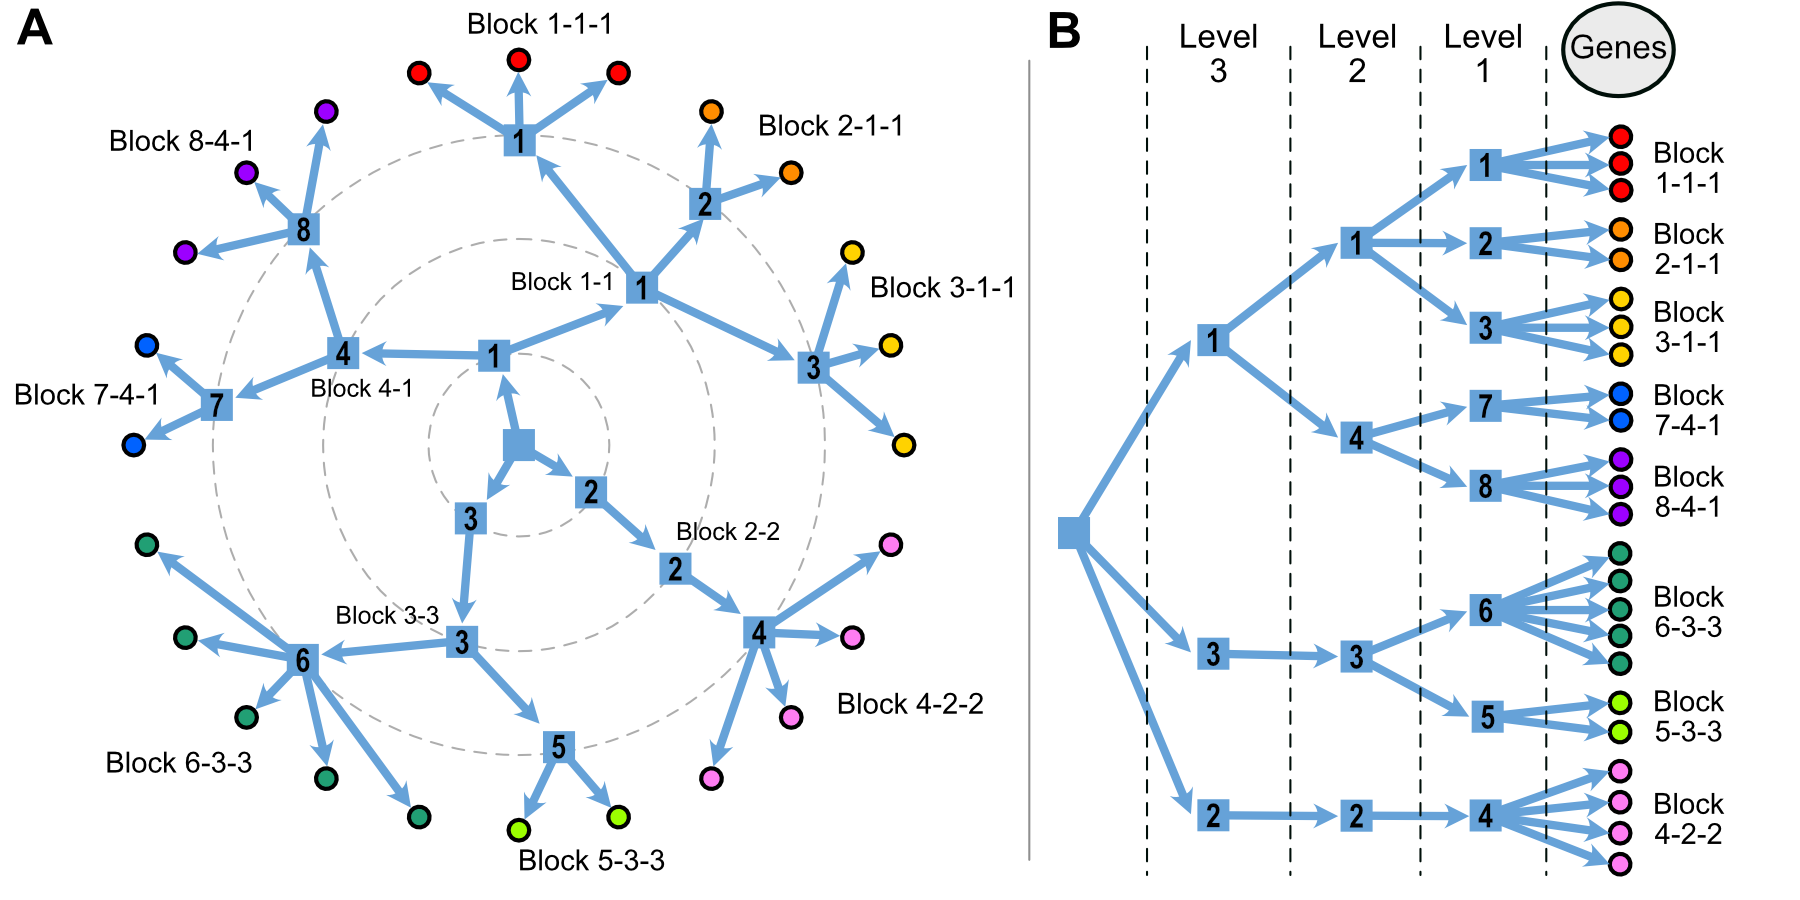
\includegraphics[width=\textwidth,height=10cm]{figures/SBM_panel_diagram.png}
\caption{Schematic representation of the clustering in the SBM. Genes
are clustered into level-1 blocks, level-1 blocks are clustered into
level-2 blocks, and so on. A. Circular representation of the clustering
we use in the following figures. Block names are constructed by
following the hierarchy, starting at level 1. So in this example, the
level-1 block 8 can also be referred to as 8-4-1. B. A tree-like
representation that highlights the hierarchy in the nested SBM. Each
level-2 block is composed of all the genes in its child level-1 blocks,
each level-3 block is composed of all the genes in its child level-2
blocks, and so on.}\label{fig:SBM_diagram}
\end{figure}

\subsubsection{Modularity and
Assortativity}\label{modularity-and-assortativity}

Although the nested SBM does not attempt to find the partition of genes
that maximizes modularity (see definition below), when using this method
we can ask if the inferred partition is modular or not by calculating
the Newman modularity at each level of the hierarchy. Newman Modularity
is calculated at each nested level using:

\[
Q = \frac{1}{2E} \sum_r e_{rr} - \frac{e_{r}^2}{2E}
\]

where \(e_{rr}\) is, by convention, twice the sum of edge weights
internal to group \(r\), \(e_{rs}\) is the sum of edge weights between
groups \(r\) and \(s\), \(e_{r} = \sum_s  e_{rs}\), and \(E\) is the sum
of all weights. Newman modularity quantifies the intuition that genes in
the same module should be more connected than across modules by
comparing the within-group connections (\(e_{rr}\)) to the expected
value of the connections across all the groups (\(\frac{e_{r}^2}{2E}\)).
The higher the difference between correlations within- and
between-groups, the higher the value of \(Q\).

We follow {[}\citeproc{ref-Peixoto2018-or}{14}{]} and further decompose
the contribution of each Level-1 block to the modularity by defining the
local assortativity of a block as:

\[
q_r = \frac{B}{2E} \left ( e_{rr} - \frac{e_{r}^2}{2E} \right )
\]

where \(B\) is the number of blocks. Using this definition, modularity
is just the average local assortativity,
\(Q = \frac{1}{B} \sum_r  q_r\). Blocks with a positive value of \(q_r\)
show assortativity, while blocks with negative values of \(q_r\) show
dissortativity, with more connections across other blocks than within.
We note that \(q_r\) values are not independent, and changes in the
assortativity of one block can lead to changes in assortativity for the
other blocks. Furthermore, the possible values of modularity for a
particular network depend on other aspects of the network other than the
community structure, like degree distribution, and therefore comparisons
of modularity values across different networks should be made with
caution {[}\citeproc{ref-Cinelli2020-tx}{28}{]}. Even so, if we consider
that the modularity value \(Q\) is meaningfully estimated, the \(q_r\)
values can be interpreted as the contribution of each block to the total
modularity.

\subsection{WGCNA}\label{wgcna}

We use WGCNA to cluster the genes into modules using the topological
overlap measure (TOM) similarity with a soft threshold of 6 in a signed
similarity measure. WGCNA produces modules by cutting the hierarchical
clustering tree at different heights, and we use the dynamic cutting
option to create the modules. We use a signed network (as opposed to
ignoring the sign of the correlation between genes) because inspection
of the gene network graph reveals large groups of genes linked by
negative correlations in our data, suggesting a large-scale structure
that would be obscured by using the unsigned method. Signed similarity
has been shown to lead to more robust modules
{[}\citeproc{ref-Mason2009-ej}{29}{]}, and in tuning WGCNA we were able
to cluster more genes and find more modules using the signed method. The
choice of using WGCNA with the full dense network and not the FDR
trimmed is intentional, as we feel it is important to compare the
methods using their recommended workflows. The use of p-value FDR
trimming is not a part of the standard WGCNA method and would be a novel
and untested modification. Additionally, WGCNA already has a strategy to
handle edges with small correlations through its use of
soft-thresholding. The way we process the gene expression data is an
integral part of the clustering method we are comparing, even if they
lead to different networks. Our intention here was to compare the full
workflow, not the specific clustering on a particular network. Given
this, we present the results using WGCNA's proposed workflow below and
add the FDR trimmed version of WGCNA to the Supporting Information (SI
Fig 2). Using the trimmed version of the network in WGCNA does not
significantly change the main results.

\begin{figure}
\centering
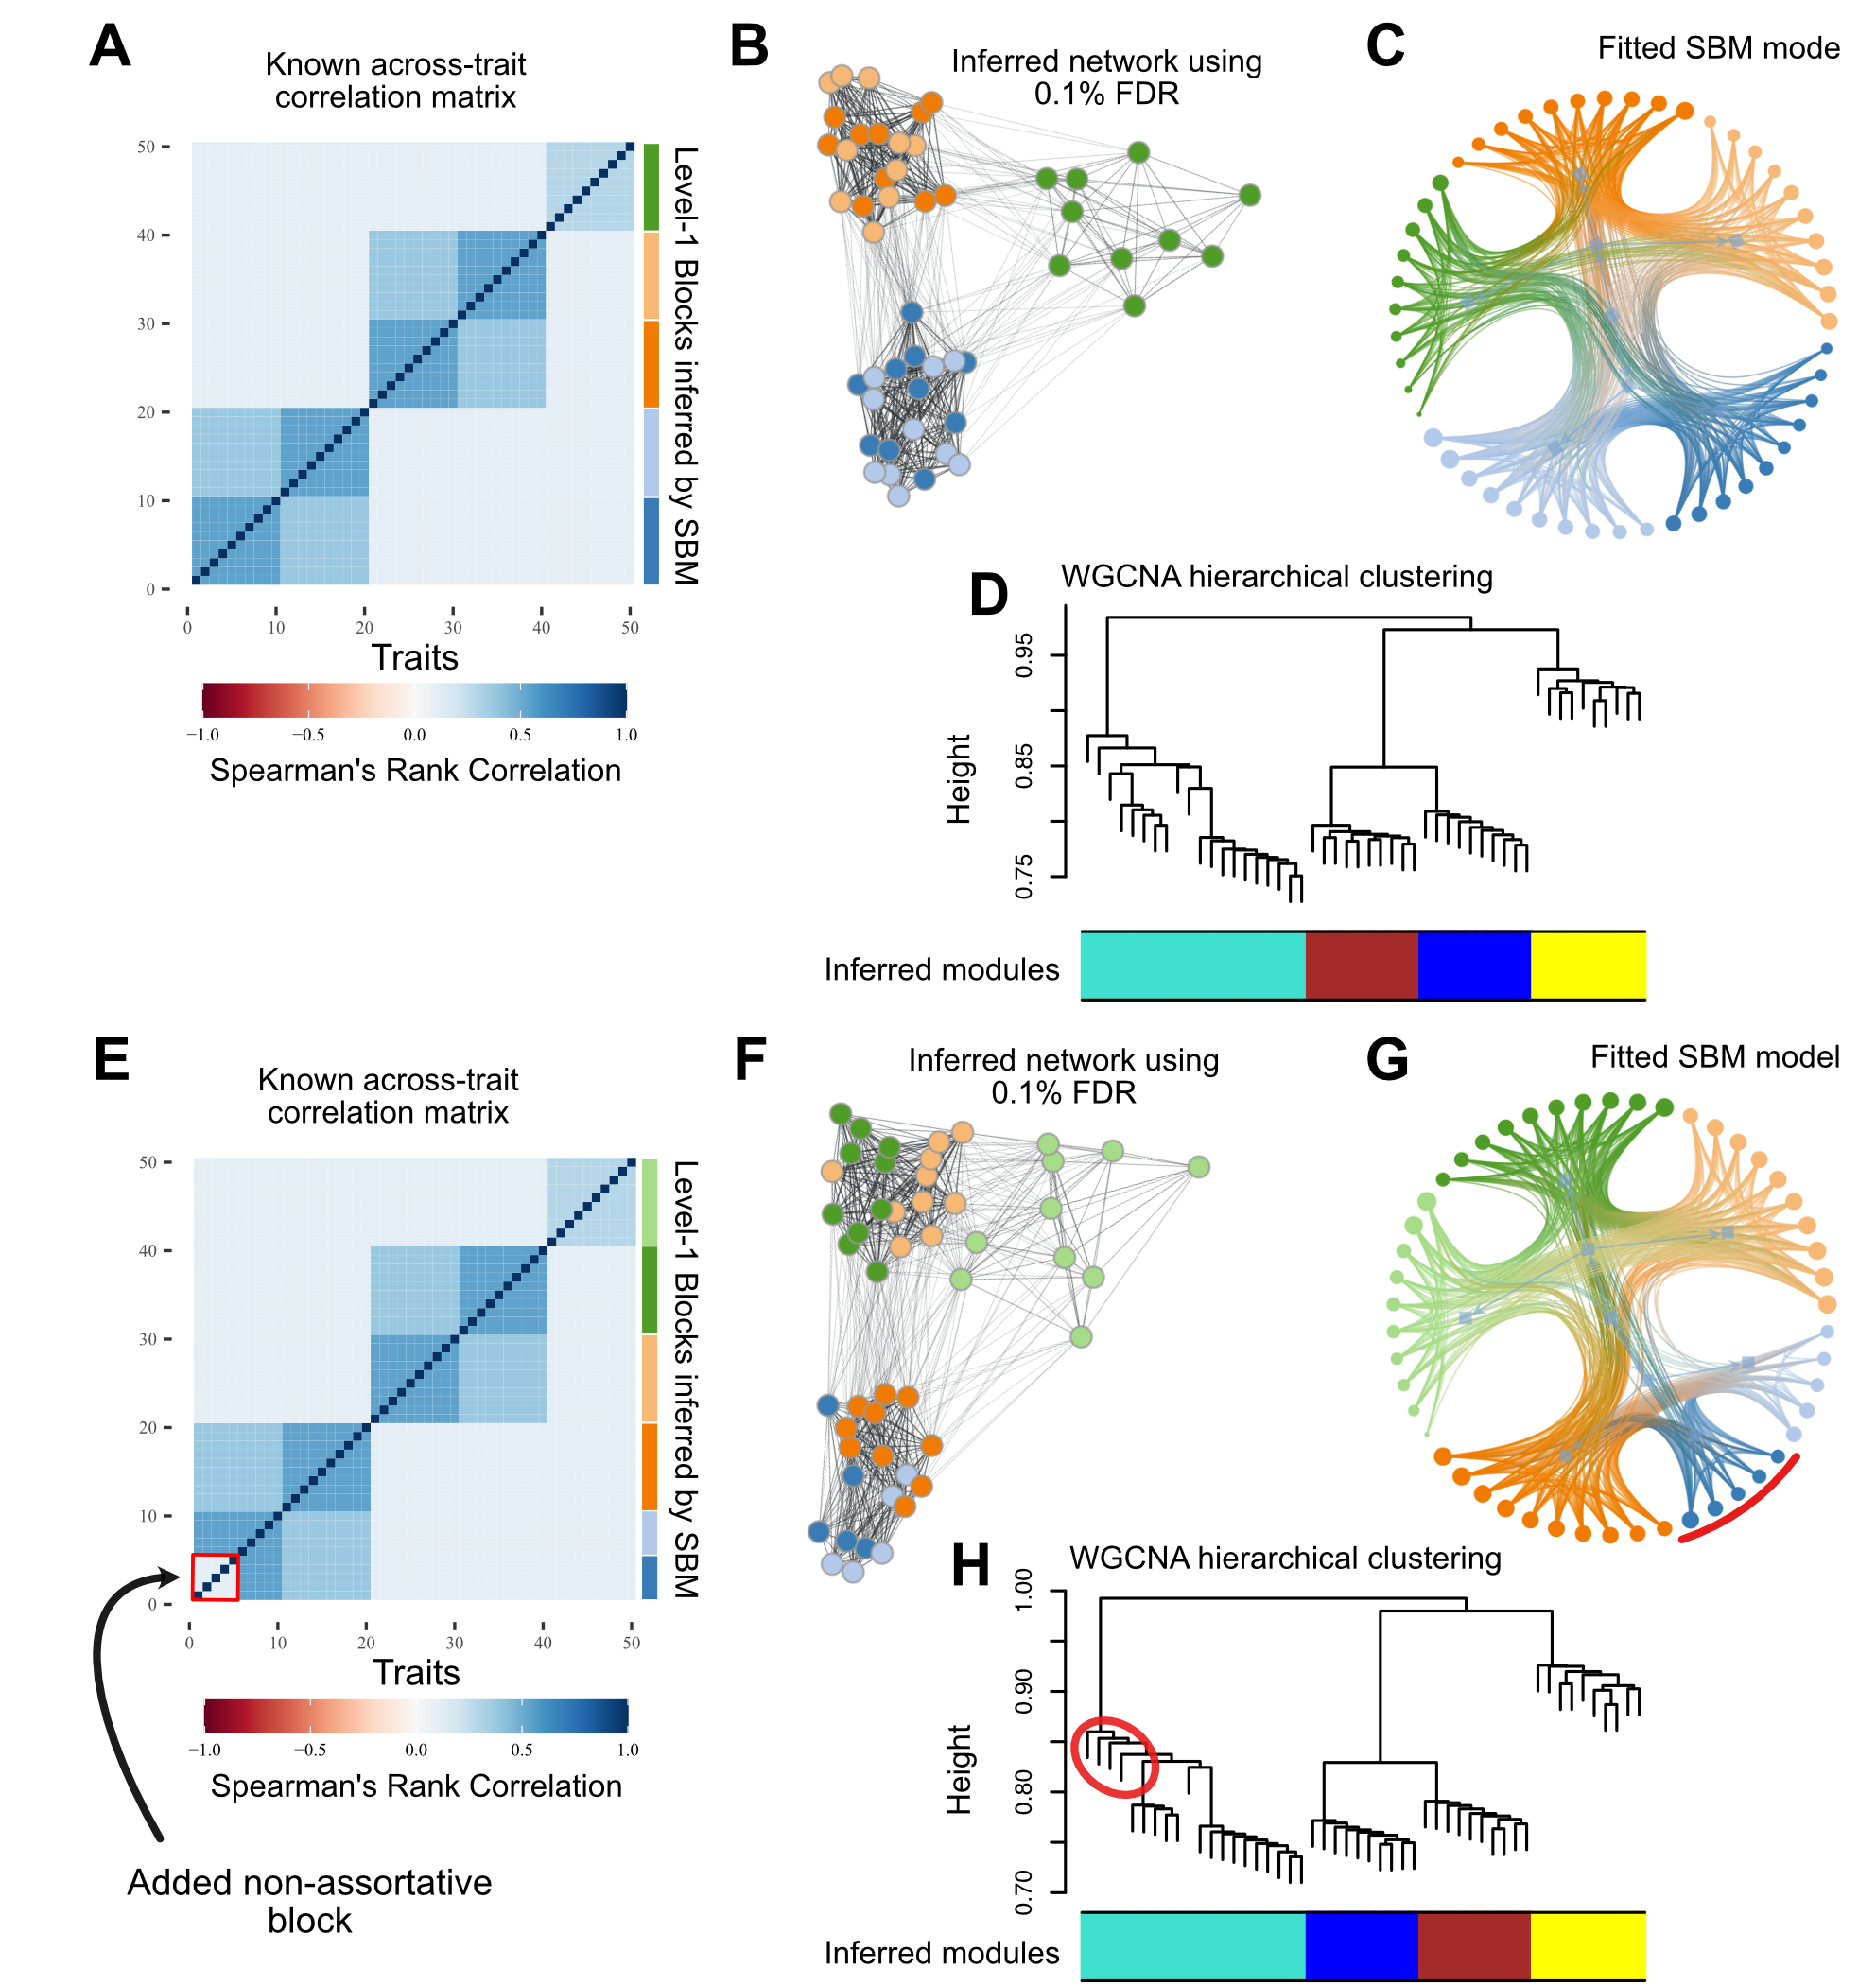
\includegraphics[width=\textwidth,height=7in]{figures/simulation_figure.png}
\caption{Simulations comparing the Stochastic Block Model (SBM) and
Weighted Gene Co-expression Network Analysis (WGCNA) in detecting
assortative and non-assortative network structure. A. Known modular
correlation matrix with 50 traits grouped into 5 assortative modules,
further organized into 2 higher-level groupings and a fifth module
equally correlated with the others. B. FDR-trimmed weighted network
generated from observations sampled from the correlation matrix in (A).
C. SBM fit on the network in (B), correctly identifying the five modules
and their higher-level organization. Edges are colored according to the
block assignment of the vertices. D. WGCNA fit on the network in (B),
detecting the only 4 assortative modules but not the higher-level
groupings. E. Modified correlation matrix with a non-assortative module
(first 5 traits, highlighted in red) introduced. F. FDR-trimmed weighted
network generated from observations sampled from the correlation matrix
in (E). G. SBM fit on the network in (F), correctly identifying the
non-assortative module (in blue with red arc) and the assortative
modules. H. WGCNA fit on the network in (F), failing to recognize the
non-assortative module and grouping its traits (circled in red) with an
assortative module (teal module). These simulations show the ability of
SBM to capture both assortative and non-assortative network structures,
as well as hierarchical organization, compared to WGCNA, which is
primarily designed for detecting assortative
communities.}\label{fig:simulations}
\end{figure}

\subsection{Simulations}\label{simulations}

Given that there are several articles using simulations to compare the
clustering obtained via SBM to other modularity maximization methods, so
we do not employ extensive simulations here. For example, see
{[}\citeproc{ref-Peixoto2023-xd}{18}{]} and references therein for an
overview of the performance of SBM in the context of inferring community
structure, and see {[}\citeproc{ref-Zhang2020-up}{19}{]} for a version
of SBM specifically developed to overcome the problems of modularity
maximization when searching for assortative communities. Instead, we use
a simple simulation to illustrate our network building and community
detection workflow and to show the different aspects of network
architecture that can be captured by both methods. We start with a known
modular correlation matrix (SI data 2), with 50 traits grouped into 5
assortative modules. These five modules are further grouped such that
there are 2 higher level groupings with two modules each, and the fifth
module is equally correlated with the other 4 (Fig~\ref{fig:simulations}
A). Using this correlation matrix, we sample 1000 draws from a
multivariate normal distribution, generating observations that follow
the known correlation pattern (SI data 2). We then measure the Spearman
correlation across these simulated observations and produce an FDR
trimmed weighted network (Fig~\ref{fig:simulations} B) that is then
clustered using SBM (Fig~\ref{fig:simulations} C) and WGCNA
(Fig~\ref{fig:simulations} D). Next, we modify the original correlation
matrix to include a non-assortative module. We accomplish this by taking
the first 5 traits and setting the correlations between them to a value
lower than the across module correlations (Fig~\ref{fig:simulations} E).
We then repeat the sampling and inference procedure, producing a new
trimmed network (Fig~\ref{fig:simulations} F), an SBM fit on this
network (Fig~\ref{fig:simulations} G), and a WGCNA fit on this network
(Fig~\ref{fig:simulations} H).

\subsection{Gene Ontology enrichment}\label{gene-ontology-enrichment}

We assess the biological relevance of the clustering obtained by each
method by comparing their gene ontology (GO) enrichment. We filter GO
enrichment p-values using a BH FDR rate of 5\%, with a minimum of 4
genes in each enriched set. All gene ontology analyses were done using
the clusterProfiler R package v4.2.2 {[}\citeproc{ref-Wu2021-db}{30}{]}
and the Org.Dm.eg.db database package v3.15
{[}\citeproc{ref-godb}{31}{]}.

\begin{longtable}[]{@{}rccccc@{}}
\caption{Fraction of blocks at each level of the SBM hierarchy that show
significant GO enrichment at the 5\% FDR level with a minimum of 4 genes
in the enriched set.}\tabularnewline
\toprule\noalign{}
Tissue & Level 1 & Level 2 & Level 3 & Level 4 & Level 5 \\
\midrule\noalign{}
\endfirsthead
\toprule\noalign{}
Tissue & Level 1 & Level 2 & Level 3 & Level 4 & Level 5 \\
\midrule\noalign{}
\endhead
\bottomrule\noalign{}
\endlastfoot
Head & 65\% (53/82) & 100\% (21/21) & 100\% (6/6) & 100\% (3/3) & 100\%
(2/2) \\
Body & 65\% (51/78) & 95\% (20/21) & 100\% (9/9) & 100\% (3/3) & 100\%
(2/2) \\
\end{longtable}

\section{Results}\label{results}

\subsection{Simulations}\label{simulations-1}

Our simulations illustrate the differences between the SBM and WGCNA in
capturing various aspects of network architecture. When applied to the
simulated data with assortative modular structure
(Fig~\ref{fig:simulations} A), both methods were able to recover the
underlying community structure to a certain extent. The SBM
(Fig~\ref{fig:simulations} C) correctly identified the five modules and
further grouped them into two higher-level clusters. WGCNA
(Fig~\ref{fig:simulations} D) detected the 4 modules, failing to
separate the first two modules. Furthermore, when a non-assortative
group was introduced into the correlation matrix
(Fig~\ref{fig:simulations} E), the two methods exhibited markedly
different behaviors with respect to this non-assortative group. The SBM
(Fig~\ref{fig:simulations} G) was able to identify the non-assortative
cluster (highlighted in red) and correctly assigned its traits to a
separate block, showing its ability to detect various types of network
structures beyond assortative communities. In contrast, WGCNA
(Fig~\ref{fig:simulations} H) failed to recognize the non-assortative
module and instead grouped its traits with one of the assortative
modules (colored in teal), highlighting its limitation in handling
non-assortative network architectures. Indeed, there is no way for the
hierarchical tree to identify this group as a separate cluster. These
results underscore the versatility of the SBM in capturing diverse
network architectures, including both assortative and non-assortative
modules, as well as hierarchical organization.

The simulations also illustrate the effectiveness of the FDR-based
network trimming approach in reducing network density while preserving
biologically relevant connections. The trimmed networks
(Fig~\ref{fig:simulations} panels B and F) maintained the essential
structure of the original correlation matrices while removing
potentially spurious edges that we lack the statistical power to
identify.

\subsection{Gene clustering}\label{gene-clustering}

To assess the consequences of assuming that communities in
transcriptional are networks assortative, we compared the performance of
a clustering algorithm that relies on assortativity (WGCNA) to the
performance of the SBM. For this, we run both clustering algorithms on
the same gene co-expression matrices. To distinguish between gene
clusters derived from the SBM and WGCNA, we refer to the former as
`blocks', and to the latter as `modules'. Gene clustering for all
methods is presented in Supporting Information Table S1.

Using the SBM, in both head and body, we were able to cluster all genes,
identifying a nested partition with 5 levels (Fig~\ref{fig:Emats}). We
obtain 2 blocks for both tissues at level 5 (the coarsest); 3 blocks for
both tissues at level 4; 6 block for the head and 9 blocks for the body
in level 3; 21 blocks for both tissues at level 2; and, finally, 82
blocks for the head and 78 blocks for the body at level 1. In what
follows, when discussing specific SBM blocks, we either explicitly
define which level of the nested hierarchy we are referring to or give
the full path to a given block. For example, level-1 block 12 can also
be referred to as 12-7-2-2-1 (see Fig~\ref{fig:SBM_diagram} for an
illustration on how to interpret these labels).

In contrast with the SBM, WGCNA was able to cluster only 30-40\% of the
genes. These 2118 genes in the body and 1600 genes in the head were
partitioned into 7 modules in both tissues. To assess whether the gene
clusters inferred by each algorithm are similar, we compared the results
of WGCNA to the SBM blocks at level 3 (Fig~\ref{fig:wgcna_compare}). We
focused on level 3 instead of level 1 (the finest level) because the
number of blocks at this level (6 in the head and 9 in the body) are
similar to the number of modules in WGCNA (7 modules for both tissues).
Overall, the partitions are different, but WGCNA and the SBM do capture
some common signals, evidenced by the tendency of Level-3 blocks that
share the same Level-4 blocks to be grouped into the same modules in
WGCNA. For example, Level-3 blocks 0, 2, 5, and 6 in the body are split
between modules 3 and 4, and these blocks are all in the same Level-4
block 0, suggesting some similarity that could explain the WGCNA
clustering. Blocks 7 and 9 are both fully assigned to module 2. Also in
the body, we find a similar pattern for Level-3 blocks 1, 3, and 4,
which are mostly split between modules 1 and 2. In the head, Level-3
block 4 is all assigned to modules 1 and 3. Level-3 blocks 1 and 2 are
mostly split between modules 1 and 3, and both are in Level-4 block 2.
Importantly, level 3 is an intermediate level in the clustering
hierarchy resolved by the SBM, and at finer levels (i.e., level 2 and 1)
the gene groups are smaller and functionally more specific.

\begin{figure}
\centering
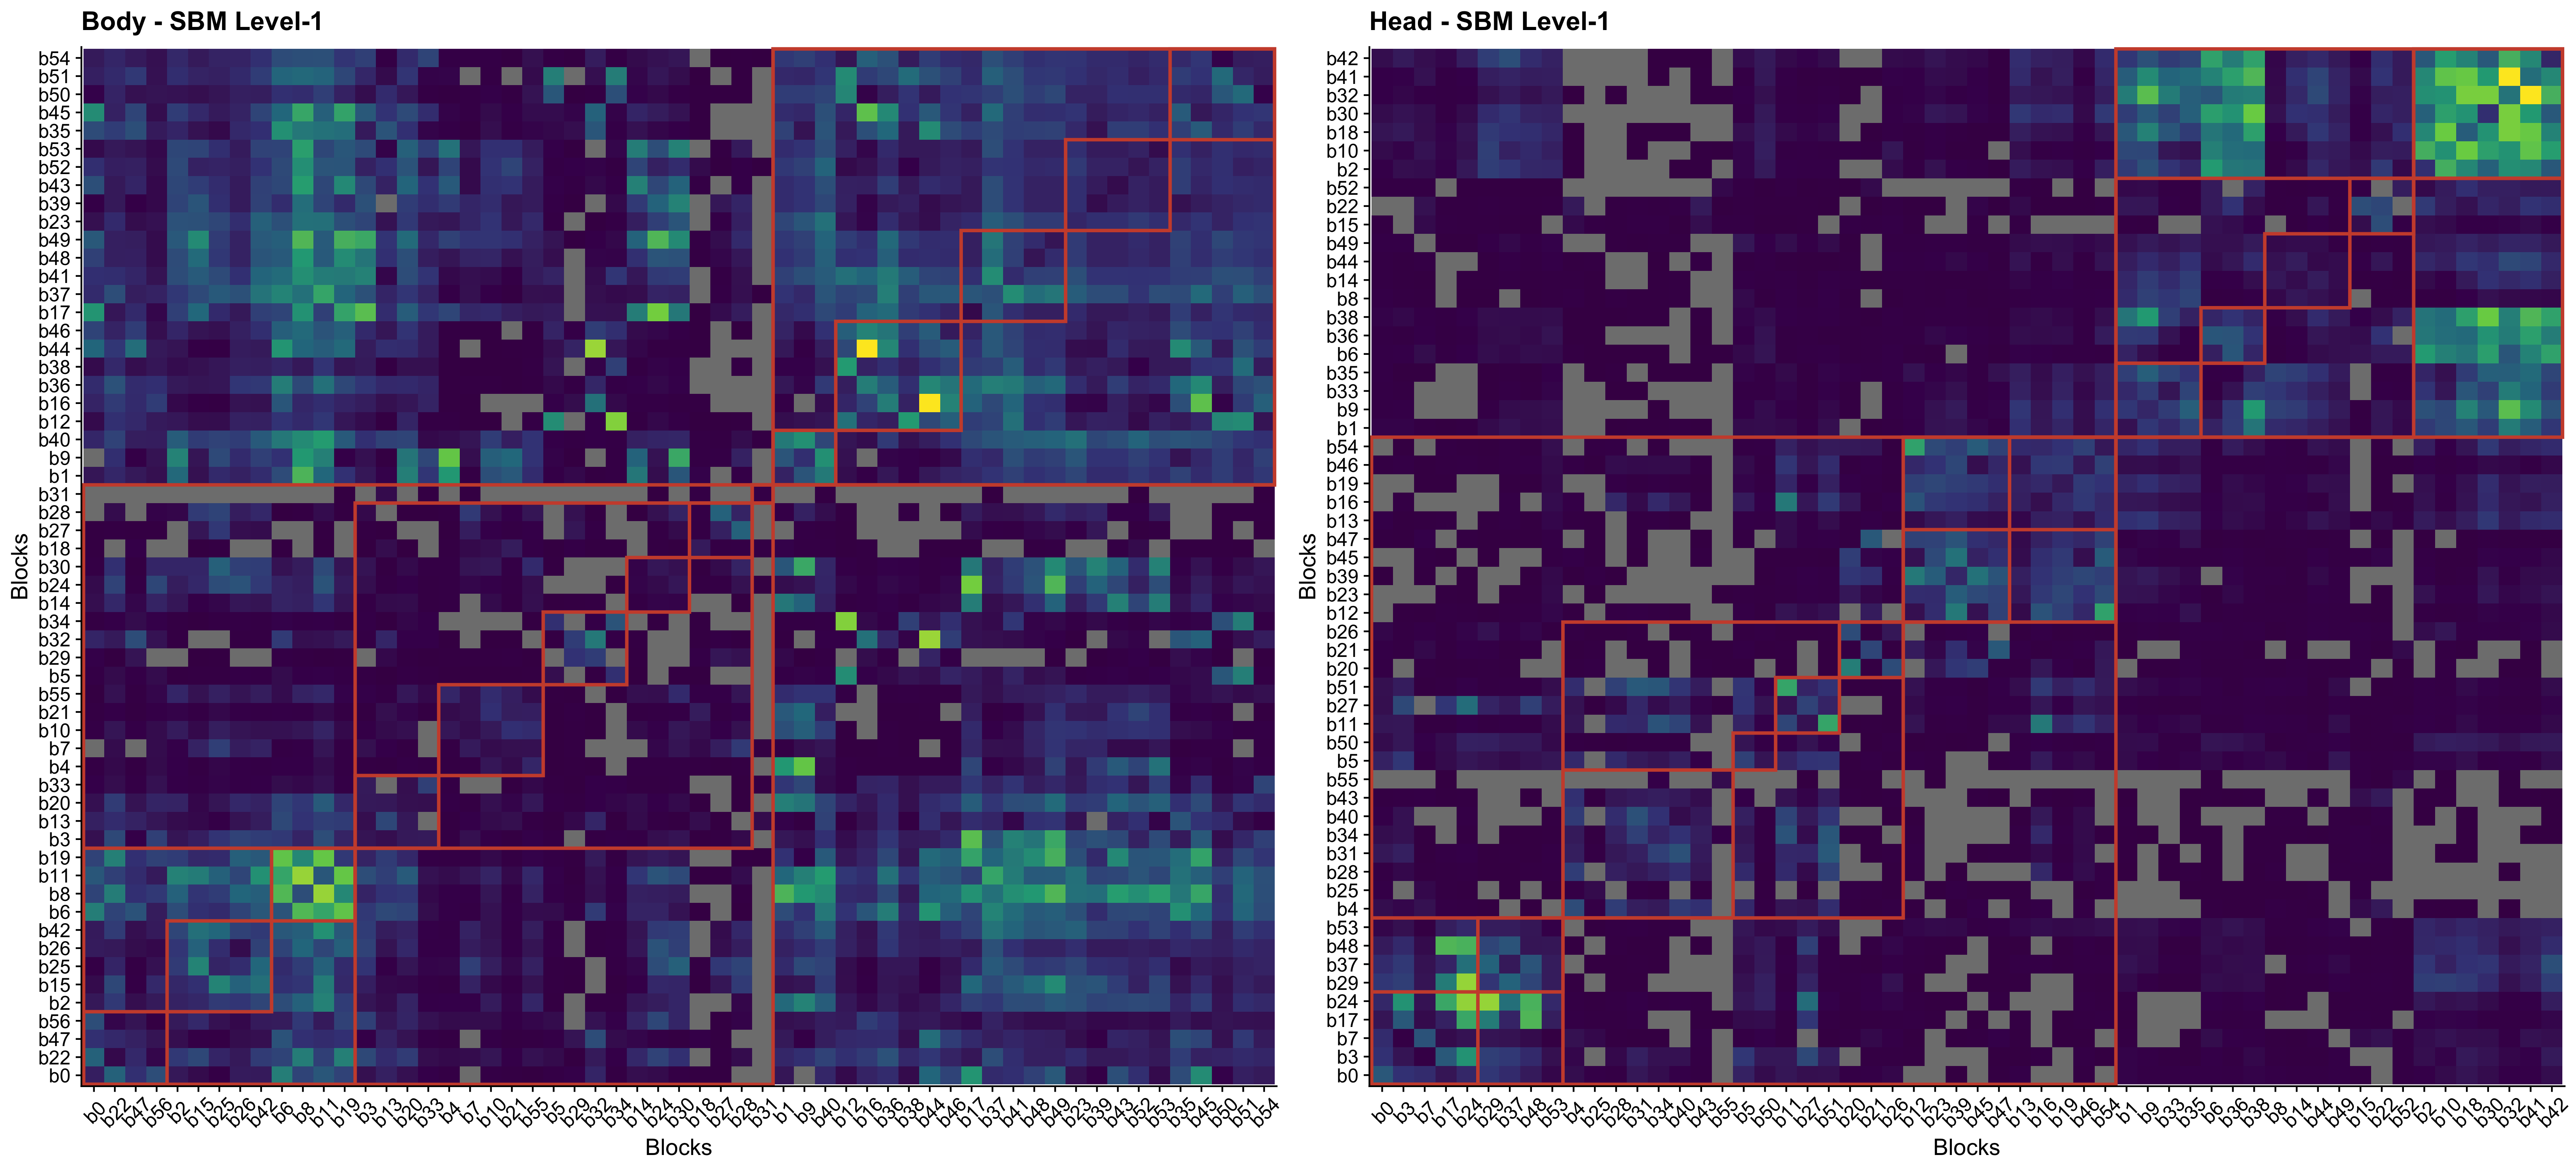
\includegraphics{figures/SBM_Ematrix.png}
\caption{Matrix and graph representations of the SBM clustering. A and
B: SBM Level-1 blocks are colored by the number of edges within and
between blocks. Gray squares represent pairs of unconnected blocks. The
upper levels of the nested hierarchy are shown by the red lines. C and
D: A full representation of the fitted block model. Genes are shown at
the perimeter, colored by their level 2 blocks. The internal graph shows
the hierarchical structure of the fitted SBM. Numbers in blue circles
correspond to the level-2 block. Arrows between level-1 blocks and genes
are omitted, unlike fig.~1. A subsample of 30.000 edges is shown
connecting the genes, and edges are colored according to their
transformed weights, with more positive weights plotted on top and more
yellow. External labels refer to a non-exhaustive subset of level-2
blocks with clear biological functions inferred from interpreting GO
enrichment. Level-2 block 8 in the body, with the blue circle
highlighted in red, is the only level-2 block with no GO
enrichment.}\label{fig:Emats}
\end{figure}

\begin{figure}
\centering
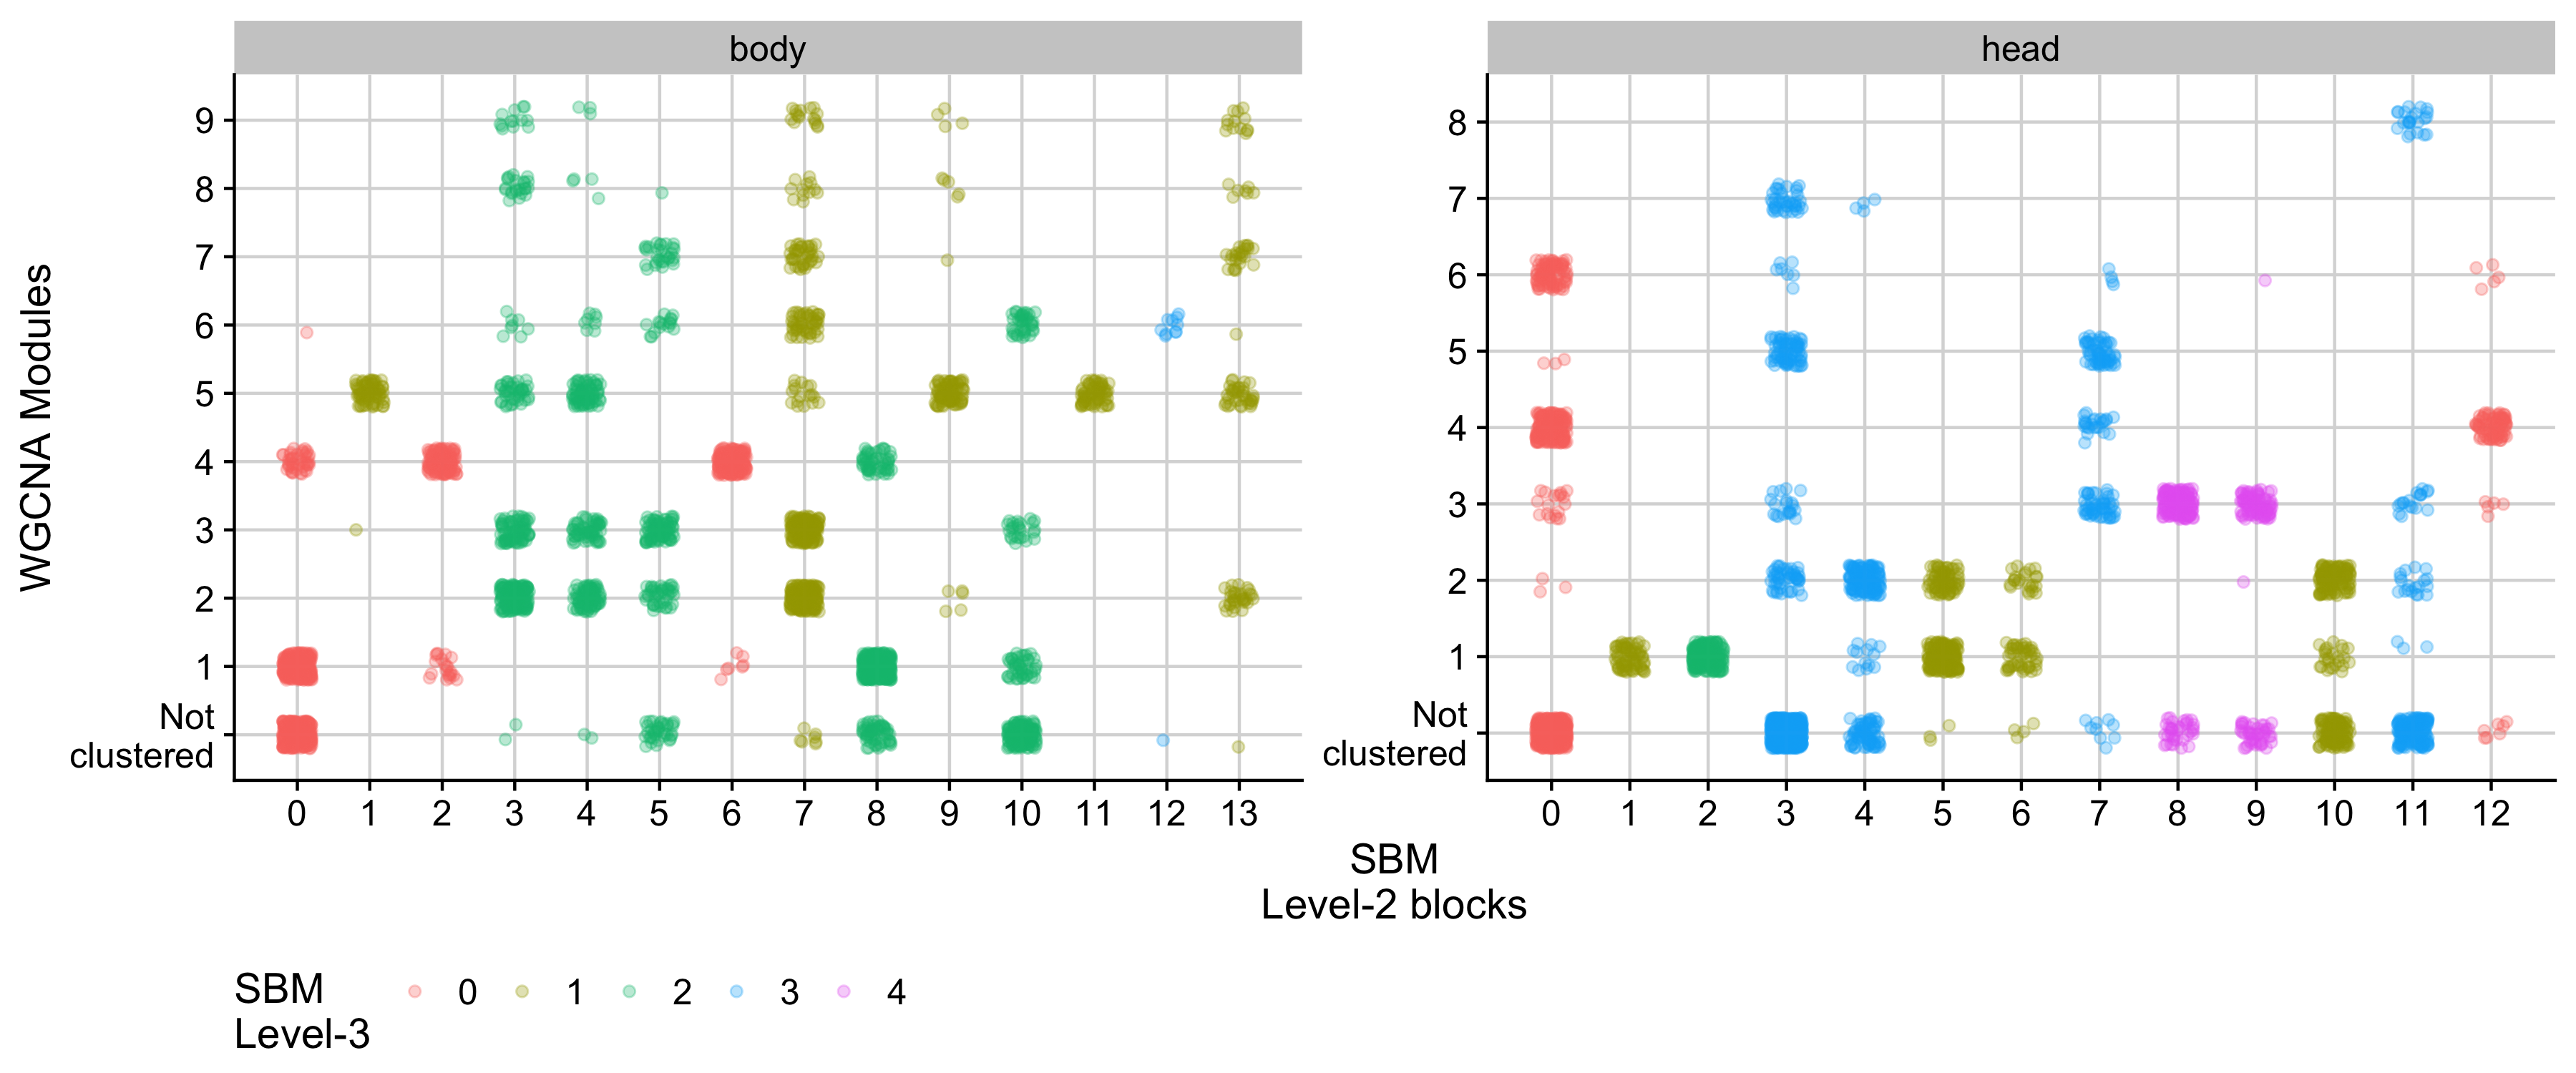
\includegraphics{figures/WGCNA_comparison.png}
\caption{Comparison of the clustering in WGCNA and levels 3 and 4 of the
SBM hierarchy for the gene expressions in the body (left) and the head
(right). Each point corresponds to a gene. The x-axis corresponds to the
Level-3 SBM blocks, and the y-axis the WGCNA modules. Colors correspond
to the (coarser) level 4 of the SBM.}\label{fig:wgcna_compare}
\end{figure}

\subsection{Modularity and
assortativity}\label{modularity-and-assortativity-1}

Because the SBM does not use modularity maximization to find
communities, we were able to use the resulting clustering to measure, in
an unbiased manner, the assortativity of individual blocks and the
overall degree of modularity of the transcriptional networks in the head
and the body. We find that modularity and assortativity are markedly
lower in the body (Fig~\ref{fig:modularity}). Several blocks in the body
have negative assortativity (being more connected across blocks than
within), and the maximum value of modularity is 0.035 at level 4 of the
nested hierarchy. Even so, several blocks show GO enrichment throughout
the distribution of assortativity. In the head, overall modularity is
higher, with a peak at 0.14 in level 3. This is still a relatively low
value and illustrates how assuming the gene network should be modular
can prevent us from finding an informative clustering. All but 5 blocks
in the head show positive assortativity, and again GO enrichment is
present throughout the assortativity range (Fig~\ref{fig:modularity}).

\begin{figure}
\centering
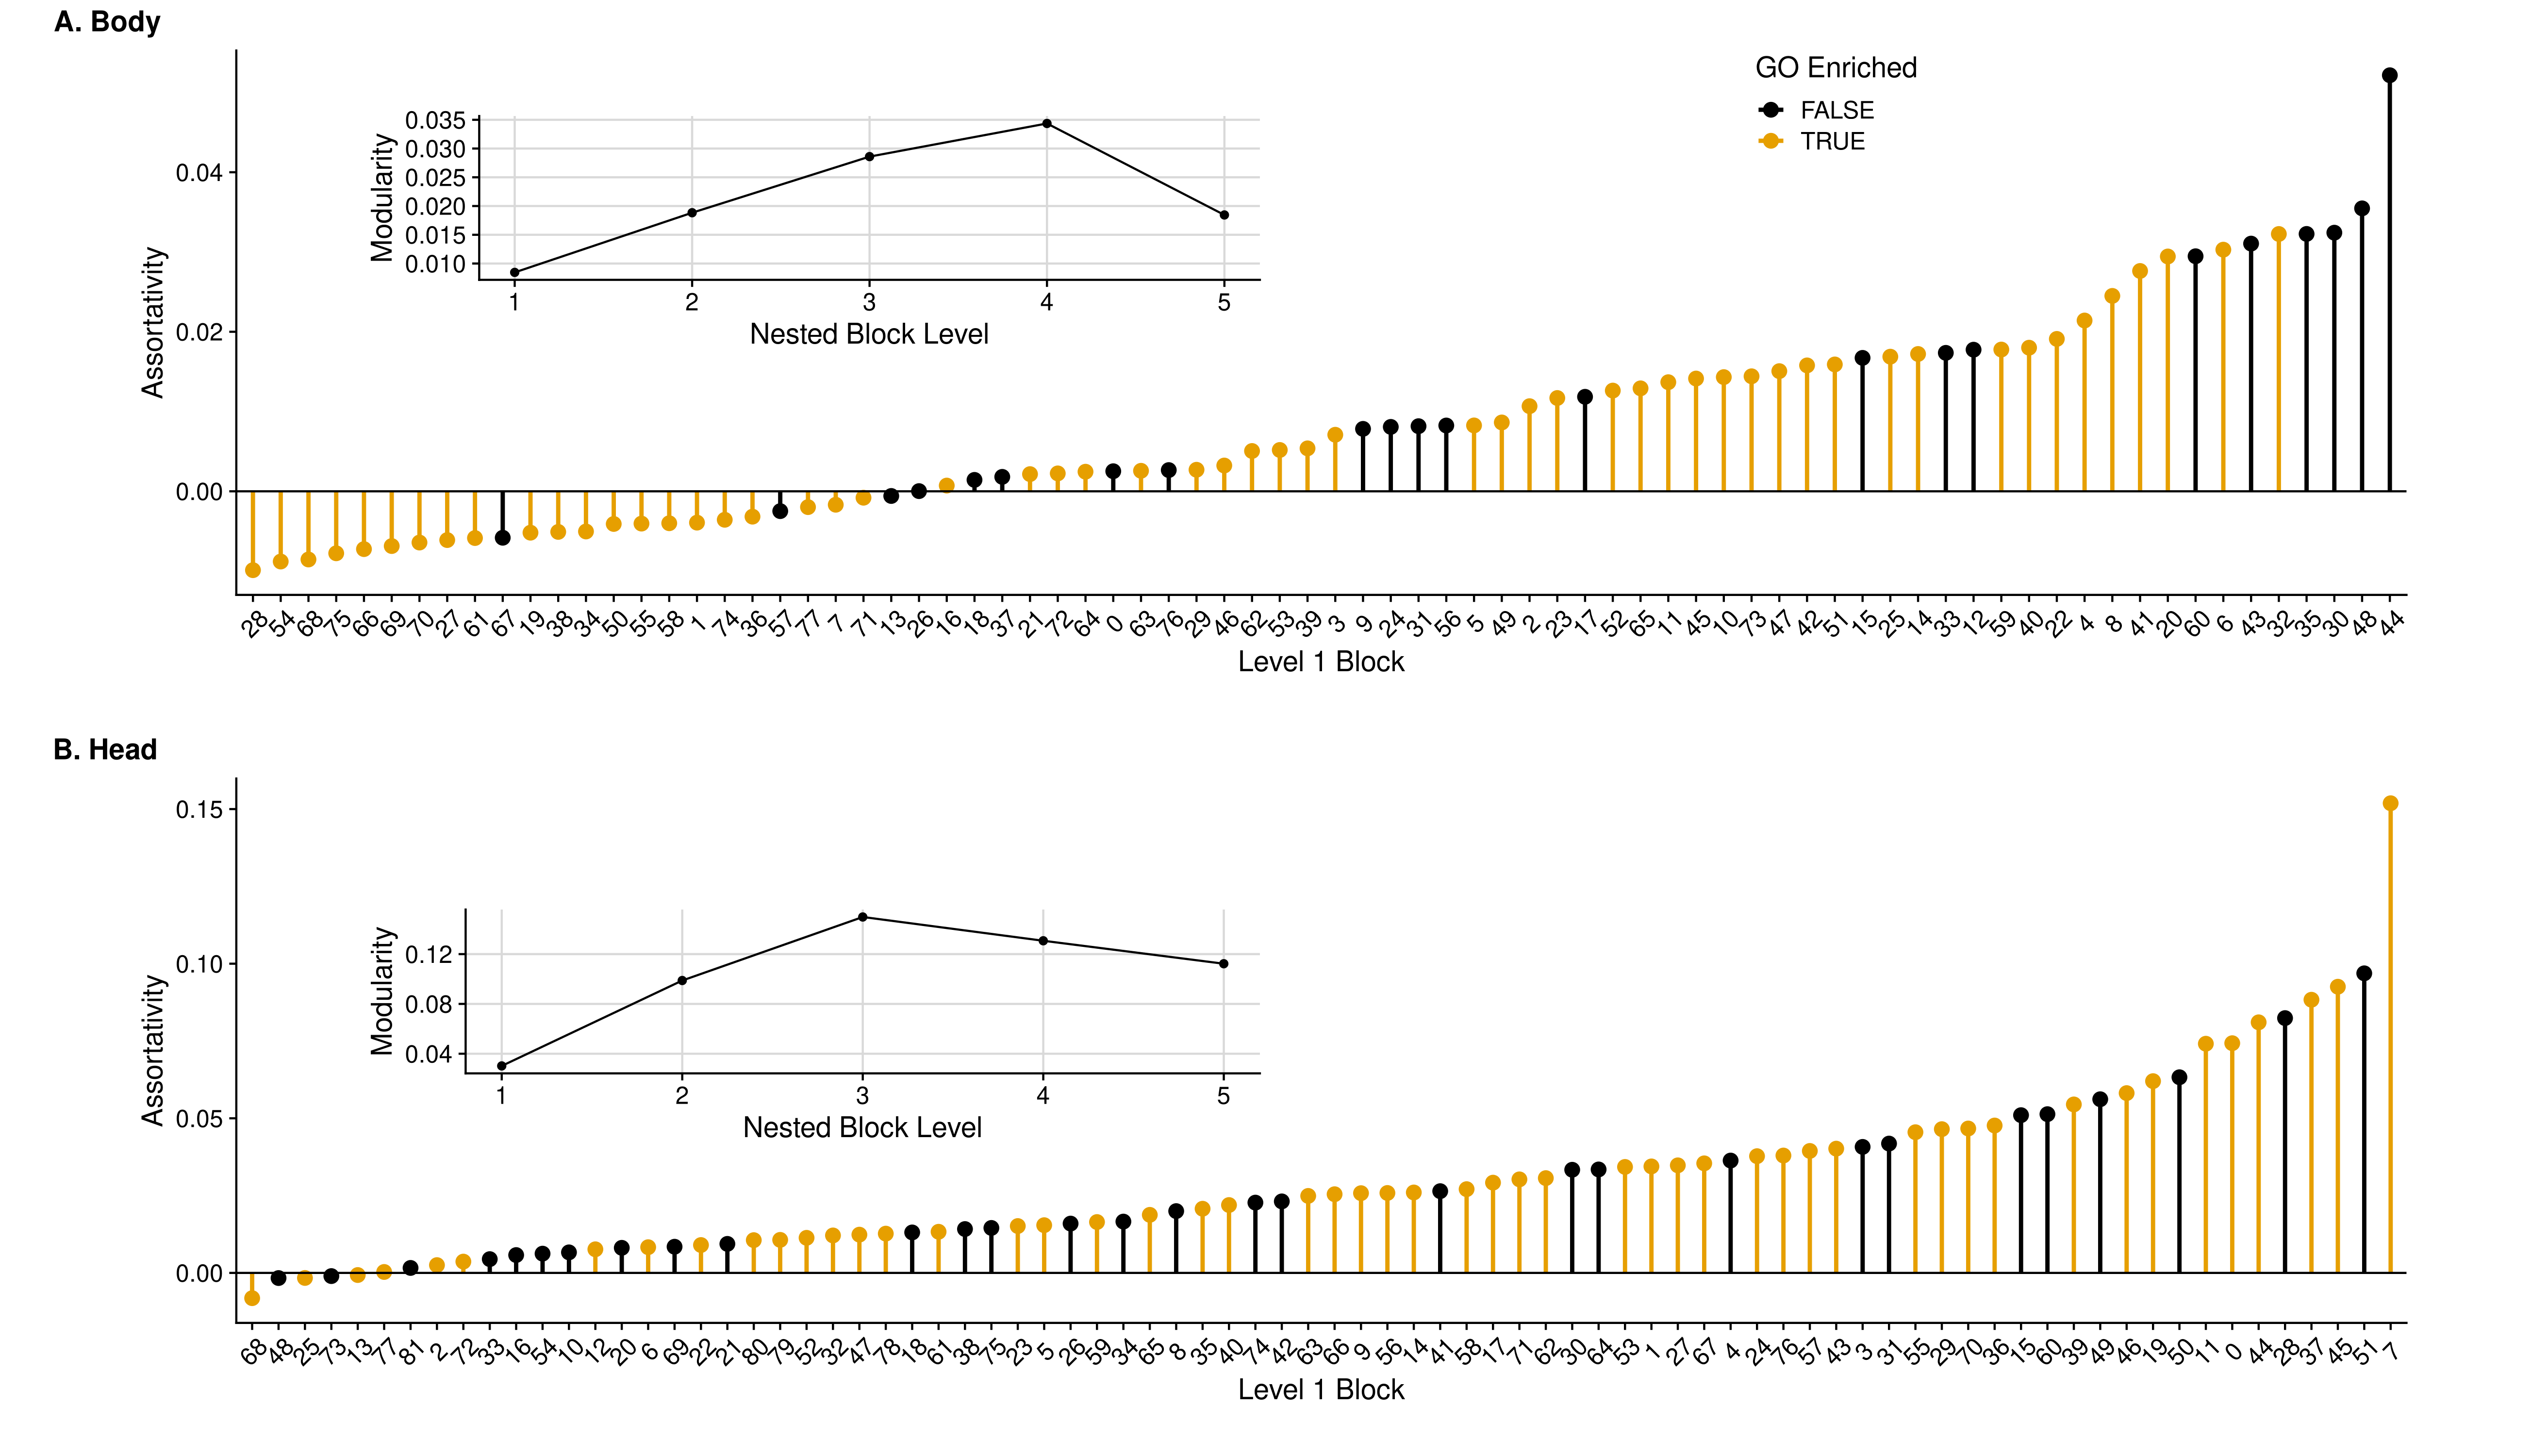
\includegraphics{figures/assortativity.png}
\caption{Assortativity measured in the SBM level-1 blocks and Newman
Modularity (average assortativity) at each level of the SBM hierarchy
(inset). GO enriched blocks are shown in yellow and appear throughout
the distribution of assortativity. Modularity is much higher in the
head, and it peaks at level 3, dropping in upper levels. Body has a much
higher number of non-assortative blocks and lower modularity at all
levels. Modularity peaks at level 4 in the body and drops strongly at
level 5. Interestingly, the 4 most assortative blocks in the body do not
show significant GO enrichment.}\label{fig:modularity}
\end{figure}

\subsection{Gene Ontology enrichment}\label{gene-ontology-enrichment-1}

Most blocks in SBM show significant GO enrichment (Table 1). Enriched
level-1 blocks show between 1 and 202 enriched terms, with a mean of 24
terms and median of 13 terms. Level-2 blocks show between 2 and 297
enriched terms, with a mean of 58 terms and median of 38 terms.
Furthermore, several blocks show remarkable consistency in their
enrichment. For example, Level-3 block 0 in the head is related to
neural signaling, sensory perception, and signal transduction. Examining
lower levels of the hierarchy, we see that often the daughter blocks at
Level-2 are also enriched with generally similar terms, as expected, but
these tend to become more specific as we go down the hierarchy. For
example, Level-2 blocks 4 and 6: (4-0-0-0) G protein-coupled receptor
signaling pathway, detection of light stimulus, phototransduction;
(6-0-0-0) synapse organization, axon development, cell-cell signaling,
behavior. Many of these enrichments are exclusive to one of the level-1
blocks. Most other Level-2 and Level-1 blocks are readily identifiable
as related to development, DNA transcription, cell respiration, cell
cycle regulation, immune response, sugar metabolism, among others
(Fig~\ref{fig:Emats}). All WGCNA modules show GO enrichment (but modules
5, 6, and 7 in the body show only one or two enriched terms, and could
be false positives. The more convincing specific enrichments show
several related enriched terms). The remaining modules show between 20
and 462 enriched terms, with a mean of 116 terms and median of 58 terms.
In general, these enrichments tend to be less specific than the SBM
blocks, spanning several biological processes. Supporting Information
Table S2 shows GO enrichment for all SBM blocks and WGCNA modules.

\subsubsection{Notable individual
clusters}\label{notable-individual-clusters}

Level 2 block 0-0-0 in the head is one of the easiest to interpret,
being entirely related to nervous tissue function. SI Fig 3 shows the
top 8 GO categories for each of the level-1 blocks in block 0-0-0, and
the most neuronal enriched WGCNA grouping, module 4. The SBM blocks
separate vesicle exocytosis, neuronal differentiation,
phototransduction, synaptic signaling, and, interestingly, there is a
block related to mRNA processing, which is notable given that
alternative splicing is thought to be more common in brain tissues
{[}\citeproc{ref-Su2018-nz}{32}{]}. WGCNA module 4 recovers some of this
enrichment but in a less granular way. The cell adhesion and
developmental part of the enrichment in block 0-0-0 is separated between
WGCNA modules 4 and 5. Some of the level-1 blocks shown in SI Fig 3 are
among the most assortative (above 0.03, see Fig~\ref{fig:modularity} B),
and so are prime candidates for detection in WGCNA. The alternative
splicing module has a much lower assortativity, so it is not surprising
that WGCNA could not detect it.

Some of the most specific enrichments in the SBM are the
translation-related blocks. In both body and head, ribosomal proteins
are clustered in small and highly enriched level-1 blocks: 6 level-1
blocks in the head and 11 in the body are composed of virtually only
ribosome-related protein genes. All are very small, being composed of
between 10-30 genes, have low assortativity
(Fig~\ref{fig:assort_translation}), and are enriched for very few terms,
almost all related to translation. In the body, all of these translation
blocks are grouped in level-4 block 1; in the head, they are split
between level-4 blocks 1 and 2. Both groups are visible in
Fig~\ref{fig:Emats} . There is no equivalent module in WGCNA, but all
translation-related genes are in the same much larger modules (module 2
in the head, 295 genes; and module 2 in the body, 345 genes), both of
which show enrichment for translation but also several other categories.
In the body WGCNA module 2, we see 68 enriched terms related to
translation, cell respiration, and several small molecules' metabolic
processes; in module 2 of the head tissue, we see 35 enriched terms
related to translation, cell respiration, and muscle development. The
level-2 clustering of level-1 blocks in the SBM is also informative. In
the head, all the translation level-1 blocks are in their own level-2
blocks (8-4-1-1, 7-2-2-1, and 2-2-2-1). In contrast, in the body, the
level-1 translation blocks sometimes share level-2 blocks with cell
respiration blocks: 1-7-1-1 is composed exclusively of level-1 blocks
related to translation, but block 14-9-1-1 is split into translation and
mitochondrial respiration level-1 blocks. WGCNA also places cell
respiration-related genes in the body on the same module 2.

\begin{figure}
\centering
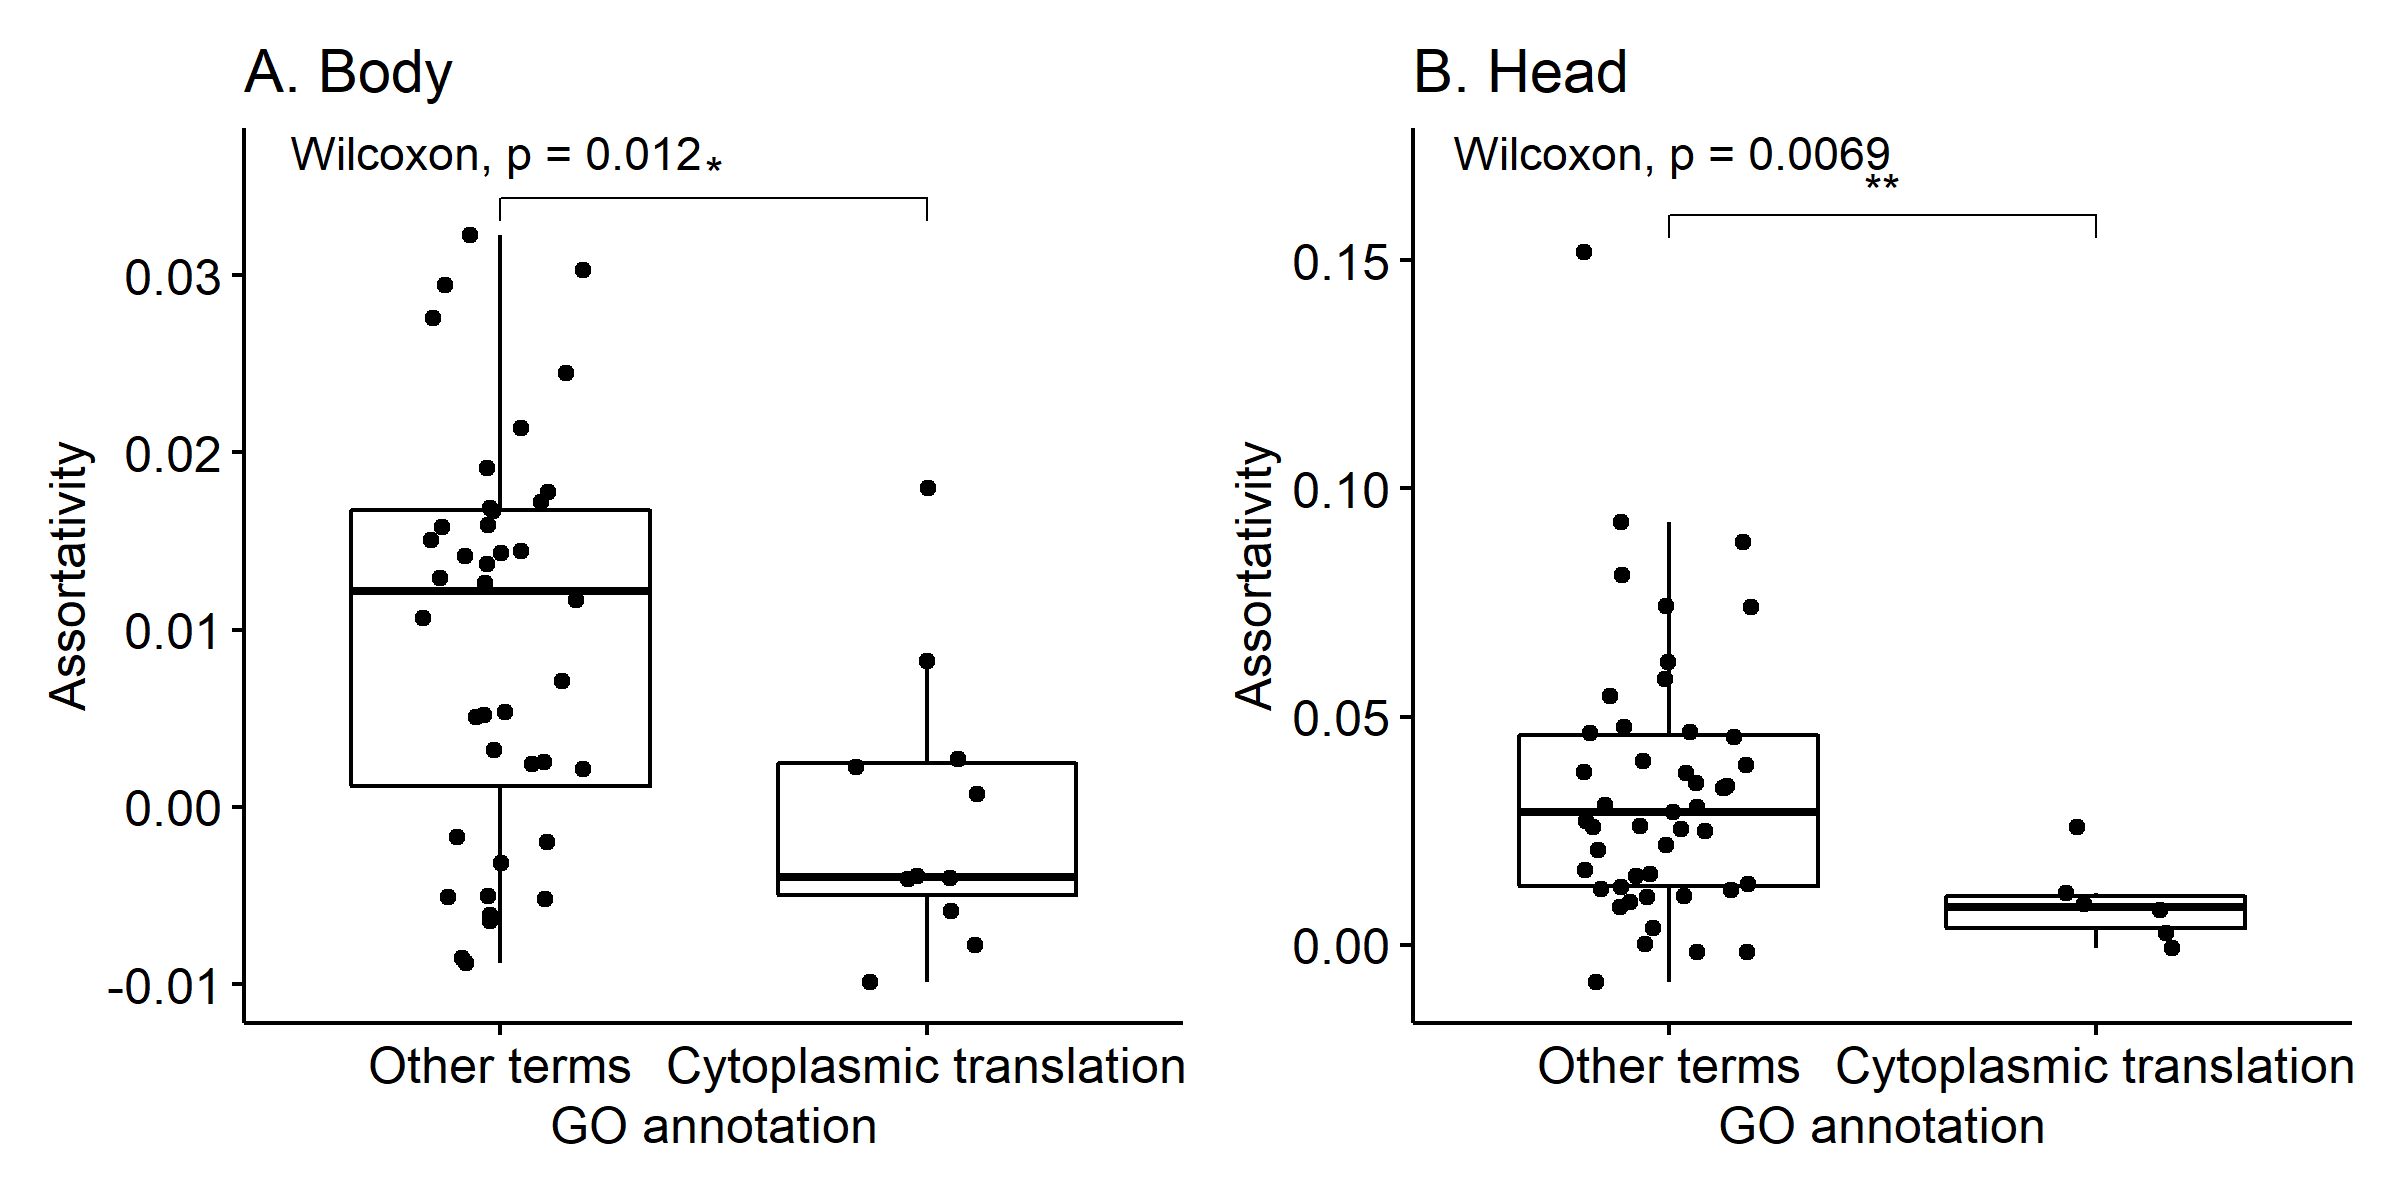
\includegraphics{figures/assortativity_cytoplasmic_translation.png}
\caption{Comparison of assortativity values between level-1 blocks
enriched for cytoplasmic translation and all other blocks. Blocks
enriched for cytoplasmic translation tend to be less
assortative.}\label{fig:assort_translation}
\end{figure}

\section{Discussion}\label{discussion}

Here, we have used the Stochastic Block Model to explore the
organization of gene co-expression networks in female \emph{Drosophila
melanogaster}. The SBM, in contrast with other gene clustering methods,
clusters genes by finding groupings that capture as much information on
the network of interactions as possible, and was able to (i) cluster all
genes into blocks; (ii) identify blocks with both, high resolution (few
genes per block) and high functional content (significant GO
associations); and (iii) identify blocks that are assortative (higher
within- than between-block correlation) as well as non-assortative. This
last point exemplifies the novelty of the SBM approach. Using the SBM
implies a shift on how we explore co-expression networks: instead of
assuming the network is modular and clustering genes based on this
assumption, we uncover clusters based on their information content and
ask if the resulting groups are modular. Surprisingly, the answer is not
always.

\subsection{Community detection
methods}\label{community-detection-methods}

The other clustering approaches we use, that explicitly search for
assortative modules, carry important downsides. Methods that use
modularity maximization (WGCNA
{[}\citeproc{ref-Langfelder2008-qa}{3}{]}, MCMC
{[}\citeproc{ref-Stone2009-hv}{11}{]}) are subject to know statistical
problems, surprisingly being prone to both overfitting (finding modular
community structure where there is none,
{[}\citeproc{ref-Guimera2004-jq}{25}{]}) and under-fitting (failing to
find modular structure), due to a problem known as the resolution limit,
which causes small modules to be incorrectly clustered together in large
networks {[}\citeproc{ref-Fortunato2007-ao}{33}{]}. Using WGCNA involves
manually tuning several parameters: the choice of using a hard or soft
threshold, the exponent in the threshold, the method of separating the
genes included in the hierarchical clustering into the modules. These
are free parameters that can drastically change the number of genes that
are clustered and the number and size of modules. For tuning these
parameters, the WGCNA workflow leans heavily on the expectation that
gene co-expression networks should be approximately scale-free
{[}\citeproc{ref-Dong2007-ff}{9},\citeproc{ref-Bergmann2004-vw}{34},\citeproc{ref-Jeong2000-xe}{35}{]},
but, despite its popularity, this expectation might be unwarranted
{[}\citeproc{ref-Broido2019-hg}{36}--\citeproc{ref-Keller2005-nf}{39}{]}.
Even with optimal parameters, WGCNA often fails to assign a substantial
proportion of genes to any module. While WGCNA is rightfully popular and
efficient in finding hub genes, if some functional gene group does not
have a hub or has low average similarities, this group will never be
identified. Both limitations potentially leave biological insight on the
table by ignoring network structures that are different from what the
method expects. In contrast, all the freedom in the SBM is restricted to
the creation of the network, which we discuss below, and no assumption
is made on the structure of the communities in the network. The
clustering procedure is completely parameter free, and choices regarding
how to model the weights between edges can be made by selecting the
model with the shortest description length
{[}\citeproc{ref-Peixoto2017-zw}{15}{]}. This is a significant advantage
for applying the SBM in domains where we lack relevant domain expertise
and can't easily tune the parameters for the other clustering methods.
Furthermore, the SBM finds a much larger number of communities that are
guaranteed to be statistically supported, greatly improving the
resolution of the clustering and allowing for more precise biological
interpretation of the resulting blocks.

One aspect we did not explore here is the estimation of the gene
co-expression network itself, before any attempt at finding communities.
Both methods used weighted networks: fully connected ones for the WGCNA
(as per this methods' suggested workflow) and a sparser network for the
SBM model fitting. Estimating these weights (gene expression
correlations) is an error-prone process, as we are estimating many more
weights than we have measured individuals, leading to potentially poor
estimates {[}\citeproc{ref-Schafer2005-ld}{40}{]}. WGCNA uses a
soft-threshold approach to mitigate the impact of small correlations,
where the correlation values are raised to a power (the soft-threshold
parameter) to reduce the influence of weak correlations and emphasize
strong ones. This soft-thresholding helps to alleviate the effect of
noisy or spurious correlations in the network construction process. The
FDR edge trimming approach used in this study is an attempt to maintain
only edges for which we have sufficient evidence to include in the
network. In contrast, the more widely used correlation value
thresholding involves setting a fixed threshold for the absolute value
of the correlation coefficient, below which edges are removed from the
network. This approach can be problematic because it does not account
for the statistical significance of the correlations and may lead to the
removal of biologically relevant, but weak, edges. FDR trimming, on the
other hand, provides a less binary way of deciding which edges to
include in the network, balancing the need to control for false
positives while still retaining edges that are likely to represent
relevant associations, even if their correlation values are not
particularly high. While the procedures we used here are commonplace,
there are more principled ways of building co-expression networks
{[}\citeproc{ref-Peel2022-bq}{41}{]}, and this is an aspect of the usual
transcriptomics workflow that could potentially see massive improvements
in the near future. Methods like the graphical lasso have been used in
this context
{[}\citeproc{ref-Lingjaerde2021-fp}{42}--\citeproc{ref-Lyu2018-ac}{44}{]},
and the expectation is that, when compared to fully connected or
thresholded networks, these inferred networks should provide much better
estimates of gene-gene connections and weights. Additionally, it is
possible to combine community detection via the SBM with network
inference, simultaneously using information about community structure to
inform the network inference and vice-versa
{[}\citeproc{ref-Peixoto2019-cj}{45}{]}.

\subsection{Modularity in gene co-expression
networks}\label{modularity-in-gene-co-expression-networks}

Beyond the methodological and practical advantages discussed above, the
fact that the SBM does not find gene clusters by attempting to maximize
their modularity has major implications for our understanding of
biological networks, as it allows us to \emph{measure} the modularity of
a given network. In doing so, we find that \emph{D. melanogaster}
transcriptomes are organized into assortative as well as non-assortative
gene clusters. The latter, however, could not have been identified by
methods that assume assortative modules. The possibility of quantifying,
in a continuous scale, the degree of assortativity of each gene block
allowed us to compare the gene co-expression networks derived from head
and body tissue, and uncover marked differences in their overall degree
of modularity.

These results warrant a discussion about the origin of the assumption
that gene expression networks are modular. Modularity, understood as the
relative independence between groups of complex traits, is often invoked
to explain the evolvability of complex phenotypes and has functioned as
a unifying concept at several levels of organization with great success
{[}\citeproc{ref-Wagner2007-jt}{7},\citeproc{ref-Melo2016-yw}{46},\citeproc{ref-Zelditch2021-ue}{47}{]}.
Traits in an organism need to have some level of integration, of
interdependence, to form a functioning individual. This necessary
interaction between parts poses a problem for understanding the
evolution of complex traits, as interdependencies are expected to lead
to important evolutionary restrictions
{[}\citeproc{ref-Orr2000-gn}{48}{]}. Modularity provides a simple
solution to this problem as it allows organisms to maintain their
function unchanged by coordinating simultaneous evolutionary changes in
all related traits while keeping unrelated traits undisturbed
{[}\citeproc{ref-Ancel2000-vt}{49}--\citeproc{ref-Wagner1996-ui}{52}{]}.
The conceptual usefulness of modularity has informed much of our
thinking on how complex traits should be structured, producing a large
body of literature dedicated to finding modules and testing for their
existence {[}\citeproc{ref-Esteve-Altava2017-ws}{53}{]}. A large part of
the literature on modularity developed in the context of morphological
traits, and morphological traits being organized into modules can be
interpreted as a consequence of the very concrete structural and
developmental constraints that lead to the formation and allow proper
functioning of these individual body elements
{[}\citeproc{ref-Shirai2010-co}{54},\citeproc{ref-Marcucio2011-nq}{55}{]}.
These constraints are easy to visualize, as morphological traits like
bones and muscle have to fit together in order to function, and
individuals in which perturbations are large enough to disrupt these
couplings are not viable. The result is a modularity pattern that is
kept stable by these structural and functional constraints
{[}\citeproc{ref-Cheverud2004-ov}{56}--\citeproc{ref-Porto2009-pi}{58}{]}.
However, no such clear structural and physical constraints exist on gene
expression, and the interaction between groups of genes can happen
through more dynamic and varied mechanisms. While we might expect
related genes to be co-expressed and therefore highly correlated,
non-linear phenomena can lead to a complete decoupling of the expression
levels of co-expressed genes. For example, the effect of gene A on gene
B could have a saturation point after which increasing expression of
gene A no longer leads to higher levels of gene B, and no correlation is
detected in this regime, even if the genes are co-expressed
{[}\citeproc{ref-Cai2023-mb}{59}{]}. The marked difference in the level
of modularity across the two tissues in our samples illustrates just how
variable modularity can be, even within the same species, sex, and
population. Furthermore, modularity is not a necessary feature of
biological organization {[}even in the case of evolvability, see
\citeproc{ref-Hansen2003-fh}{60},\citeproc{ref-Roseman2009-kk}{61},\citeproc{ref-Pavlicev2011-xm}{62}{]},
and only searching for modularity can blind us to alternative
organizations, as we have shown. Indeed, the profound interconnectedness
of gene regulation networks has led to a small revolution in our
understanding of disease and complex traits
{[}\citeproc{ref-Boyle2017-re}{63}{]}. The very high dimensionality of
gene co-expression networks also allows for genes to be similar in ways
that do not lead to high correlations. For example, two genes might be
connected to the same genes in different communities, but not among
themselves (like the non-assortative block in Fig~\ref{fig:simulations}
E). This similarity would likely be missed by modularity maximization or
hierarchical clustering because these genes would not form a classic
assortative unit. Meanwhile, the SBM would correctly identify these
genes connecting two modules as being similar due to their shared
connectivity pattern. Having access to these types of blocks, which are
real but non-assortative, could bring new insight into the organization
of gene co-expression networks, illustrated by the relation we describe
between non-assortativity and cytoplasmic translation.

\subsection{Conclusion}\label{conclusion}

Here, we find that non-modular blocks are widespread in gene
co-expression networks, and that the evidence for their functional
relevance is as strong as for modular blocks. This highlights the need
to incorporate other sources of information, beyond assortativity, when
exploring biological networks. More studies using methods that don't
rely on modularity maximization will be needed to determine whether
there are general patterns of non-modular organization.

\subsection{Supporting information}\label{supporting-information}

Supporting information can be found at
\url{https://github.com/diogro/SBM_manuscript}. Code for using
graph-tools to cluster expression data using the SBM can be found at
\url{https://github.com/ayroles-lab/SBM-tools}

\begin{enumerate}
\def\labelenumi{\arabic{enumi}.}
\item
  SI Data 1 -- VOOM transformed, batch corrected, gene expression levels
\item
  SI Data 2 -- Data related to the simulations in figure 2
\item
  SI Figure 1 -- Exploration of the effect of FDR choice in the SBM
  clustering
\item
  SI Figure 2 -- WGCNA clustering using FDR trimming
\item
  SI Figures 3 -- Enriched GO categories in a level-3 block in the head
  (0-0-0), related to neural signaling.
\item
  SI table 1 -- Gene clustering using SBM and WGCNA
\item
  SI table 2 -- GO enrichment for all methods and tissues.
\item
  SI table 3 -- Summary statistics for all SBM blocks.
\end{enumerate}

\section{Author Contributions}\label{author-contributions}

\textbf{Conceptualization}: D.M., L.P., and J.A. \textbf{Data Curation}:
L.P. \textbf{Formal Analysis}: D.M. \textbf{Funding Acquisition}: D.M.,
L.P., and J.A. \textbf{Investigation}: D.M., L.P., and J.A.
\textbf{Methodology}: D.M., and L.P. \textbf{Project Administration}:
J.A. \textbf{Resources}: J.A. \textbf{Software}: D.M., and L.P.
\textbf{Supervision}: J.A. \textbf{Validation}: D.M.
\textbf{Visualization}: D.M. \textbf{Writing -- Original Draft
Preparation}: D.M. \textbf{Writing -- Review \& Editing}: D.M., L.P.,
and J.A.

\section{Acknowledgments}\label{acknowledgments}

We thank all members of the Ayroles lab for their support. We thank
Monique Simon and Cara Weisman for their thoughtful comments on an
earlier version of the manuscript. We also thank Tiago Peixoto for help
in using graph-tool. D.M. is funded by a fellowship from the Princeton
Presidential Postdoctoral Research Fellows Program. L.P. was funded by a
Long-Term Postdoctoral Fellowship from the Human Frontiers Science
Program and is funded by the Max Planck Society. J.A. is funded by
grants from the NIH: National Institute of Environmental Health Sciences
(R01-ES029929) and National Institute of General Medical Sciences
(NIGMS) (R35GM124881). This study was supported in part by the
Lewis-Sigler Institute for Integrative Genomics at Princeton University.
We also acknowledge that the work reported in this paper was
substantially performed using the Princeton Research Computing resources
at Princeton University which is a consortium of groups led by the
Princeton Institute for Computational Science and Engineering (PICSciE)
and Office of Information Technology's Research Computing.

\section*{References}\label{references}
\addcontentsline{toc}{section}{References}

\phantomsection\label{refs}
\begin{CSLReferences}{0}{1}
\bibitem[\citeproctext]{ref-Van_Dam2018-nf}
\CSLLeftMargin{1. }%
\CSLRightInline{Dam S van, Võsa U, Graaf A van der, Franke L, Magalhães
JP de. Gene co-expression analysis for functional classification and
gene-disease predictions. Brief Bioinform. 2018;19: 575--592.
doi:\href{https://doi.org/10.1093/bib/bbw139}{10.1093/bib/bbw139}}

\bibitem[\citeproctext]{ref-Dhaeseleer2005-jv}
\CSLLeftMargin{2. }%
\CSLRightInline{D'haeseleer P. How does gene expression clustering work?
Nat Biotechnol. 2005;23: 1499--1501.
doi:\href{https://doi.org/10.1038/nbt1205-1499}{10.1038/nbt1205-1499}}

\bibitem[\citeproctext]{ref-Langfelder2008-qa}
\CSLLeftMargin{3. }%
\CSLRightInline{Langfelder P, Horvath S. {WGCNA}: An {R} package for
weighted correlation network analysis. BMC Bioinformatics. 2008;9: 559.
doi:\href{https://doi.org/10.1186/1471-2105-9-559}{10.1186/1471-2105-9-559}}

\bibitem[\citeproctext]{ref-Imenez_Silva2017-ic}
\CSLLeftMargin{4. }%
\CSLRightInline{Imenez Silva PH, Melo D, Mendonça POR de. Insights from
systems biology in physiological studies: Learning from context. Cell
Physiol Biochem. 2017;42: 939--951.
doi:\href{https://doi.org/10.1159/000478648}{10.1159/000478648}}

\bibitem[\citeproctext]{ref-Olson1958-fh}
\CSLLeftMargin{5. }%
\CSLRightInline{Olson EC, Miller RL. Morphological integration. Chicago,
IL: University of Chicago Press; 1958. }

\bibitem[\citeproctext]{ref-Magwene2001-an}
\CSLLeftMargin{6. }%
\CSLRightInline{Magwene PM.
\href{https://www.ncbi.nlm.nih.gov/pubmed/11681729}{New tools for
studying integration and modularity}. Evolution. 2001;55: 1734--1745. }

\bibitem[\citeproctext]{ref-Wagner2007-jt}
\CSLLeftMargin{7. }%
\CSLRightInline{Wagner GP, Pavlicev M, Cheverud JM. {The road to
modularity}. Nat Rev Genet. 2007;8: 921--931.
doi:\href{https://doi.org/10.1038/nrg2267}{10.1038/nrg2267}}

\bibitem[\citeproctext]{ref-Zhang2005-kh}
\CSLLeftMargin{8. }%
\CSLRightInline{Zhang B, Horvath S. A general framework for weighted
gene co-expression network analysis. Stat Appl Genet Mol Biol. 2005;4:
Article17.
doi:\href{https://doi.org/10.2202/1544-6115.1128}{10.2202/1544-6115.1128}}

\bibitem[\citeproctext]{ref-Dong2007-ff}
\CSLLeftMargin{9. }%
\CSLRightInline{Dong J, Horvath S. Understanding network concepts in
modules. BMC Syst Biol. 2007;1: 24.
doi:\href{https://doi.org/10.1186/1752-0509-1-24}{10.1186/1752-0509-1-24}}

\bibitem[\citeproctext]{ref-Newman2006-fv}
\CSLLeftMargin{10. }%
\CSLRightInline{Newman MEJ. {Modularity and community structure in
networks}. Proceedings of the National Academy of Sciences. 2006;103:
8577--8582.
doi:\href{https://doi.org/10.1073/pnas.0601602103}{10.1073/pnas.0601602103}}

\bibitem[\citeproctext]{ref-Stone2009-hv}
\CSLLeftMargin{11. }%
\CSLRightInline{Stone EA, Ayroles JF. Modulated modularity clustering as
an exploratory tool for functional genomic inference. PLoS Genet.
2009;5: e1000479.
doi:\href{https://doi.org/10.1371/journal.pgen.1000479}{10.1371/journal.pgen.1000479}}

\bibitem[\citeproctext]{ref-Betzel2018-ec}
\CSLLeftMargin{12. }%
\CSLRightInline{Betzel RF, Medaglia JD, Bassett DS. Diversity of
meso-scale architecture in human and non-human connectomes. Nat Commun.
2018;9: 346.
doi:\href{https://doi.org/10.1038/s41467-017-02681-z}{10.1038/s41467-017-02681-z}}

\bibitem[\citeproctext]{ref-Peel2018-ai}
\CSLLeftMargin{13. }%
\CSLRightInline{Peel L, Delvenne J-C, Lambiotte R. Multiscale mixing
patterns in networks. Proc Natl Acad Sci U S A. 2018;115: 4057--4062.
doi:\href{https://doi.org/10.1073/pnas.1713019115}{10.1073/pnas.1713019115}}

\bibitem[\citeproctext]{ref-Peixoto2018-or}
\CSLLeftMargin{14. }%
\CSLRightInline{Peixoto TP. Nonparametric weighted stochastic block
models. Phys Rev E. 2018;97: 012306.
doi:\href{https://doi.org/10.1103/PhysRevE.97.012306}{10.1103/PhysRevE.97.012306}}

\bibitem[\citeproctext]{ref-Peixoto2017-zw}
\CSLLeftMargin{15. }%
\CSLRightInline{Peixoto TP. Nonparametric bayesian inference of the
microcanonical stochastic block model. Phys Rev E. 2017;95: 012317.
doi:\href{https://doi.org/10.1103/PhysRevE.95.012317}{10.1103/PhysRevE.95.012317}}

\bibitem[\citeproctext]{ref-Baum2019-ty}
\CSLLeftMargin{16. }%
\CSLRightInline{Baum K, Rajapakse JC, Azuaje F. Analysis of
correlation-based biomolecular networks from different omics data by
fitting stochastic block models. F1000Res. 2019;8: 465.
doi:\href{https://doi.org/10.12688/f1000research.18705.2}{10.12688/f1000research.18705.2}}

\bibitem[\citeproctext]{ref-Morelli2021-ge}
\CSLLeftMargin{17. }%
\CSLRightInline{Morelli L, Giansanti V, Cittaro D. Nested stochastic
block models applied to the analysis of single cell data. BMC
Bioinformatics. 2021;22: 576.
doi:\href{https://doi.org/10.1186/s12859-021-04489-7}{10.1186/s12859-021-04489-7}}

\bibitem[\citeproctext]{ref-Peixoto2023-xd}
\CSLLeftMargin{18. }%
\CSLRightInline{Peixoto TP. Descriptive vs. Inferential community
detection in networks: Pitfalls, myths and {Half-Truths}. Elements in
the structure and dynamics of complex networks. Cambridge University
Press; 2023.
doi:\href{https://doi.org/10.1017/9781009118897}{10.1017/9781009118897}}

\bibitem[\citeproctext]{ref-Zhang2020-up}
\CSLLeftMargin{19. }%
\CSLRightInline{Zhang L, Peixoto TP. Statistical inference of
assortative community structures. Phys Rev Research. 2020;2: 043271.
doi:\href{https://doi.org/10.1103/PhysRevResearch.2.043271}{10.1103/PhysRevResearch.2.043271}}

\bibitem[\citeproctext]{ref-Pallares2023-eQTL}
\CSLLeftMargin{20. }%
\CSLRightInline{Pallares LF, Melo D, Wolf S, Cofer EM, Varada V, Peng J,
et al. Saturating the {eQTL} map in drosophila melanogaster: Genome-wide
patterns of cis and trans regulation of transcriptional variation in
outbred populations. bioRxiv. 2023. p. 2023.05.20.541576.
doi:\href{https://doi.org/10.1101/2023.05.20.541576}{10.1101/2023.05.20.541576}}

\bibitem[\citeproctext]{ref-Pallares2020-ha}
\CSLLeftMargin{21. }%
\CSLRightInline{Pallares LF, Picard S, Ayroles JF. {TM3'seq}: A
{Tagmentation-Mediated} 3' sequencing approach for improving scalability
of {RNAseq} experiments. G3 Genes\textbar Genomes\textbar Genetics.
2020;10: 143--150.
doi:\href{https://doi.org/10.1534/g3.119.400821}{10.1534/g3.119.400821}}

\bibitem[\citeproctext]{ref-Law2014-xl}
\CSLLeftMargin{22. }%
\CSLRightInline{Law CW, Chen Y, Shi W, Smyth GK. Voom: Precision weights
unlock linear model analysis tools for {RNA-seq} read counts. Genome
Biol. 2014;15: R29.
doi:\href{https://doi.org/10.1186/gb-2014-15-2-r29}{10.1186/gb-2014-15-2-r29}}

\bibitem[\citeproctext]{ref-Leek2007-bx}
\CSLLeftMargin{23. }%
\CSLRightInline{Leek JT, Storey JD. Capturing heterogeneity in gene
expression studies by surrogate variable analysis. PLoS Genet. 2007;3:
1724--1735.
doi:\href{https://doi.org/10.1371/journal.pgen.0030161}{10.1371/journal.pgen.0030161}}

\bibitem[\citeproctext]{ref-Karrer2011-vp}
\CSLLeftMargin{24. }%
\CSLRightInline{Karrer B, Newman MEJ. Stochastic blockmodels and
community structure in networks. Phys Rev E Stat Nonlin Soft Matter
Phys. 2011;83: 016107.
doi:\href{https://doi.org/10.1103/PhysRevE.83.016107}{10.1103/PhysRevE.83.016107}}

\bibitem[\citeproctext]{ref-Guimera2004-jq}
\CSLLeftMargin{25. }%
\CSLRightInline{Guimerà R, Sales-Pardo M, Amaral LAN. Modularity from
fluctuations in random graphs and complex networks. Phys Rev E Stat
Nonlin Soft Matter Phys. 2004;70: 025101.
doi:\href{https://doi.org/10.1103/PhysRevE.70.025101}{10.1103/PhysRevE.70.025101}}

\bibitem[\citeproctext]{ref-peixoto_graph-tool_2014}
\CSLLeftMargin{26. }%
\CSLRightInline{Peixoto TP. The graph-tool python library. figshare.
2014 {[}cited 10 Sep 2014{]}.
doi:\href{https://doi.org/10.6084/m9.figshare.1164194}{10.6084/m9.figshare.1164194}}

\bibitem[\citeproctext]{ref-Kirkpatrick1983-ad}
\CSLLeftMargin{27. }%
\CSLRightInline{Kirkpatrick S, Gelatt CD Jr, Vecchi MP. Optimization by
simulated annealing. Science. 1983;220: 671--680.
doi:\href{https://doi.org/10.1126/science.220.4598.671}{10.1126/science.220.4598.671}}

\bibitem[\citeproctext]{ref-Cinelli2020-tx}
\CSLLeftMargin{28. }%
\CSLRightInline{Cinelli M, Peel L, Iovanella A, Delvenne J-C. Network
constraints on the mixing patterns of binary node metadata. Phys Rev E.
2020;102: 062310.
doi:\href{https://doi.org/10.1103/PhysRevE.102.062310}{10.1103/PhysRevE.102.062310}}

\bibitem[\citeproctext]{ref-Mason2009-ej}
\CSLLeftMargin{29. }%
\CSLRightInline{Mason MJ, Fan G, Plath K, Zhou Q, Horvath S. Signed
weighted gene co-expression network analysis of transcriptional
regulation in murine embryonic stem cells. BMC Genomics. 2009;10: 327.
doi:\href{https://doi.org/10.1186/1471-2164-10-327}{10.1186/1471-2164-10-327}}

\bibitem[\citeproctext]{ref-Wu2021-db}
\CSLLeftMargin{30. }%
\CSLRightInline{Wu T, Hu E, Xu S, Chen M, Guo P, Dai Z, et al.
clusterProfiler 4.0: A universal enrichment tool for interpreting omics
data. The Innovation. 2021;2: 100141.
doi:\href{https://doi.org/10.1016/j.xinn.2021.100141}{10.1016/j.xinn.2021.100141}}

\bibitem[\citeproctext]{ref-godb}
\CSLLeftMargin{31. }%
\CSLRightInline{Carlson M. Org.dm.eg.db: Genome wide annotation for fly.
2022. }

\bibitem[\citeproctext]{ref-Su2018-nz}
\CSLLeftMargin{32. }%
\CSLRightInline{Su C-H, D D, Tarn W-Y. Alternative splicing in
neurogenesis and brain development. Front Mol Biosci. 2018;5: 12.
doi:\href{https://doi.org/10.3389/fmolb.2018.00012}{10.3389/fmolb.2018.00012}}

\bibitem[\citeproctext]{ref-Fortunato2007-ao}
\CSLLeftMargin{33. }%
\CSLRightInline{Fortunato S, Barthélemy M. Resolution limit in community
detection. Proc Natl Acad Sci U S A. 2007;104: 36--41.
doi:\href{https://doi.org/10.1073/pnas.0605965104}{10.1073/pnas.0605965104}}

\bibitem[\citeproctext]{ref-Bergmann2004-vw}
\CSLLeftMargin{34. }%
\CSLRightInline{Bergmann S, Ihmels J, Barkai N. Similarities and
differences in genome-wide expression data of six organisms. PLoS Biol.
2004;2: E9.
doi:\href{https://doi.org/10.1371/journal.pbio.0020009}{10.1371/journal.pbio.0020009}}

\bibitem[\citeproctext]{ref-Jeong2000-xe}
\CSLLeftMargin{35. }%
\CSLRightInline{Jeong H, Tombor B, Albert R, Oltvai ZN, Barabási AL. The
large-scale organization of metabolic networks. Nature. 2000;407:
651--654. doi:\href{https://doi.org/10.1038/35036627}{10.1038/35036627}}

\bibitem[\citeproctext]{ref-Broido2019-hg}
\CSLLeftMargin{36. }%
\CSLRightInline{Broido AD, Clauset A. Scale-free networks are rare. Nat
Commun. 2019;10: 1017.
doi:\href{https://doi.org/10.1038/s41467-019-08746-5}{10.1038/s41467-019-08746-5}}

\bibitem[\citeproctext]{ref-Khanin2006-ve}
\CSLLeftMargin{37. }%
\CSLRightInline{Khanin R, Wit E. How scale-free are biological networks.
J Comput Biol. 2006;13: 810--818.
doi:\href{https://doi.org/10.1089/cmb.2006.13.810}{10.1089/cmb.2006.13.810}}

\bibitem[\citeproctext]{ref-Stumpf2005-ed}
\CSLLeftMargin{38. }%
\CSLRightInline{Stumpf MPH, Ingram PJ, Nouvel I, Wiuf C. Statistical
model selection methods applied to biological networks. Transactions on
computational systems biology {III}. Springer Berlin Heidelberg; 2005.
pp. 65--77.
doi:\href{https://doi.org/10.1007/11599128/_5}{10.1007/11599128\textbackslash\_5}}

\bibitem[\citeproctext]{ref-Keller2005-nf}
\CSLLeftMargin{39. }%
\CSLRightInline{Keller EF. Revisiting {``scale-free''} networks.
Bioessays. 2005;27: 1060--1068.
doi:\href{https://doi.org/10.1002/bies.20294}{10.1002/bies.20294}}

\bibitem[\citeproctext]{ref-Schafer2005-ld}
\CSLLeftMargin{40. }%
\CSLRightInline{Schäfer J, Strimmer K. A shrinkage approach to
large-scale covariance matrix estimation and implications for functional
genomics. Stat Appl Genet Mol Biol. 2005;4: Article32.
doi:\href{https://doi.org/10.2202/1544-6115.1175}{10.2202/1544-6115.1175}}

\bibitem[\citeproctext]{ref-Peel2022-bq}
\CSLLeftMargin{41. }%
\CSLRightInline{Peel L, Peixoto TP, De Domenico M. Statistical inference
links data and theory in network science. Nat Commun. 2022;13: 1--15.
doi:\href{https://doi.org/10.1038/s41467-022-34267-9}{10.1038/s41467-022-34267-9}}

\bibitem[\citeproctext]{ref-Lingjaerde2021-fp}
\CSLLeftMargin{42. }%
\CSLRightInline{Lingjærde C, Lien TG, Borgan Ø, Bergholtz H, Glad IK.
Tailored graphical lasso for data integration in gene network
reconstruction. BMC Bioinformatics. 2021;22: 498.
doi:\href{https://doi.org/10.1186/s12859-021-04413-z}{10.1186/s12859-021-04413-z}}

\bibitem[\citeproctext]{ref-Seal2023-qn}
\CSLLeftMargin{43. }%
\CSLRightInline{Seal S, Li Q, Basner EB, Saba LM, Kechris K. {RCFGL}:
Rapid condition adaptive fused graphical lasso and application to
modeling brain region co-expression networks. PLoS Comput Biol. 2023;19:
e1010758.
doi:\href{https://doi.org/10.1371/journal.pcbi.1010758}{10.1371/journal.pcbi.1010758}}

\bibitem[\citeproctext]{ref-Lyu2018-ac}
\CSLLeftMargin{44. }%
\CSLRightInline{Lyu Y, Xue L, Zhang F, Koch H, Saba L, Kechris K, et al.
Condition-adaptive fused graphical lasso ({CFGL)}: An adaptive procedure
for inferring condition-specific gene co-expression network. PLoS Comput
Biol. 2018;14: e1006436.
doi:\href{https://doi.org/10.1371/journal.pcbi.1006436}{10.1371/journal.pcbi.1006436}}

\bibitem[\citeproctext]{ref-Peixoto2019-cj}
\CSLLeftMargin{45. }%
\CSLRightInline{Peixoto TP. Network reconstruction and community
detection from dynamics. Phys Rev Lett. 2019;123: 128301.
doi:\href{https://doi.org/10.1103/PhysRevLett.123.128301}{10.1103/PhysRevLett.123.128301}}

\bibitem[\citeproctext]{ref-Melo2016-yw}
\CSLLeftMargin{46. }%
\CSLRightInline{Melo D, Porto A, Cheverud JM, Marroig G. Modularity:
Genes, development and evolution. Annu Rev Ecol Evol Syst. 2016;47:
463--486.
doi:\href{https://doi.org/10.1146/annurev-ecolsys-121415-032409}{10.1146/annurev-ecolsys-121415-032409}}

\bibitem[\citeproctext]{ref-Zelditch2021-ue}
\CSLLeftMargin{47. }%
\CSLRightInline{Zelditch ML, Goswami A. What does modularity mean? Evol
Dev. 2021; e12390.
doi:\href{https://doi.org/10.1111/ede.12390}{10.1111/ede.12390}}

\bibitem[\citeproctext]{ref-Orr2000-gn}
\CSLLeftMargin{48. }%
\CSLRightInline{Orr HA. Adaptation and the cost of complexity.
Evolution. 2000;54: 13--20.
doi:\href{https://doi.org/10.1111/j.0014-3820.2000.tb00002.x}{10.1111/j.0014-3820.2000.tb00002.x}}

\bibitem[\citeproctext]{ref-Ancel2000-vt}
\CSLLeftMargin{49. }%
\CSLRightInline{Ancel LW, Fontana W.
\href{https://www.ncbi.nlm.nih.gov/pubmed/11069142}{Plasticity,
evolvability, and modularity in {RNA}}. J Exp Zool. 2000;288: 242--283.
}

\bibitem[\citeproctext]{ref-Cheverud1996-jw}
\CSLLeftMargin{50. }%
\CSLRightInline{Cheverud JM. {Developmental Integration and the
Evolution of Pleiotropy}. Integr Comp Biol. 1996;36: 44--50.
doi:\href{https://doi.org/10.1093/icb/36.1.44}{10.1093/icb/36.1.44}}

\bibitem[\citeproctext]{ref-Wagner2011-zx}
\CSLLeftMargin{51. }%
\CSLRightInline{Wagner GP, Zhang J. The pleiotropic structure of the
genotype-phenotype map: The evolvability of complex organisms. Nat Rev
Genet. 2011;12: 204--213.
doi:\href{https://doi.org/10.1038/nrg2949}{10.1038/nrg2949}}

\bibitem[\citeproctext]{ref-Wagner1996-ui}
\CSLLeftMargin{52. }%
\CSLRightInline{Wagner GP, Altenberg L. Perspective: Complex adaptations
and the evolution of evolvability. Evolution. 1996;50: 967--976.
doi:\href{https://doi.org/10.2307/2410639}{10.2307/2410639}}

\bibitem[\citeproctext]{ref-Esteve-Altava2017-ws}
\CSLLeftMargin{53. }%
\CSLRightInline{Esteve-Altava B. In search of morphological modules: A
systematic review. Biol Rev Camb Philos Soc. 2017;92: 1332--1347.
doi:\href{https://doi.org/10.1111/brv.12284}{10.1111/brv.12284}}

\bibitem[\citeproctext]{ref-Shirai2010-co}
\CSLLeftMargin{54. }%
\CSLRightInline{Shirai LT, Marroig G. Skull modularity in neotropical
marsupials and monkeys: Size variation and evolutionary constraint and
flexibility. J Exp Zool B Mol Dev Evol. 2010;314: 663--683.
doi:\href{https://doi.org/10.1002/jez.b.21367}{10.1002/jez.b.21367}}

\bibitem[\citeproctext]{ref-Marcucio2011-nq}
\CSLLeftMargin{55. }%
\CSLRightInline{Marcucio RS, Young NM, Hu D, Hallgrimsson B. Mechanisms
that underlie co-variation of the brain and face. Genesis. 2011;49:
177--189.
doi:\href{https://doi.org/10.1002/dvg.20710}{10.1002/dvg.20710}}

\bibitem[\citeproctext]{ref-Cheverud2004-ov}
\CSLLeftMargin{56. }%
\CSLRightInline{Cheverud JM. Modular pleiotropic effects of quantitative
trait loci on morphological traits. In: Schlosser G G \& Wagner, editor.
Modularity in development and evolution. Chicago: University of Chicago
Press; 2004. pp. 132--153. }

\bibitem[\citeproctext]{ref-Cheverud1984-mi}
\CSLLeftMargin{57. }%
\CSLRightInline{Cheverud JM. {Quantitative genetics and developmental
constraints on evolution by selection.} J Theor Biol. 1984;110:
155--171.
doi:\href{https://doi.org/10.1016/S0022-5193(84)80050-8}{10.1016/S0022-5193(84)80050-8}}

\bibitem[\citeproctext]{ref-Porto2009-pi}
\CSLLeftMargin{58. }%
\CSLRightInline{Porto A, Oliveira FB de, Shirai LT, De Conto V, Marroig
G. {The Evolution of Modularity in the Mammalian Skull I: Morphological
Integration Patterns and Magnitudes}. Evol Biol. 2009;36: 118--135.
doi:\href{https://doi.org/10.1007/s11692-008-9038-3}{10.1007/s11692-008-9038-3}}

\bibitem[\citeproctext]{ref-Cai2023-mb}
\CSLLeftMargin{59. }%
\CSLRightInline{Cai H, Des Marais DL. Revisiting regulatory coherence:
Accounting for temporal bias in plant gene co-expression analyses. New
Phytol. 2023;238: 16--24.
doi:\href{https://doi.org/10.1111/nph.18720}{10.1111/nph.18720}}

\bibitem[\citeproctext]{ref-Hansen2003-fh}
\CSLLeftMargin{60. }%
\CSLRightInline{Hansen TF.
\href{https://www.ncbi.nlm.nih.gov/pubmed/12689723}{Is modularity
necessary for evolvability? Remarks on the relationship between
pleiotropy and evolvability}. Biosystems. 2003;69: 83--94. }

\bibitem[\citeproctext]{ref-Roseman2009-kk}
\CSLLeftMargin{61. }%
\CSLRightInline{Roseman CC, Kenney-Hunt JP, Cheverud JM. Phenotypic
integration without modularity: Testing hypotheses about the
distribution of pleiotropic quantitative trait loci in a continuous
space. Evol Biol. 2009;36: 282--291.
doi:\href{https://doi.org/10.1007/s11692-009-9067-6}{10.1007/s11692-009-9067-6}}

\bibitem[\citeproctext]{ref-Pavlicev2011-xm}
\CSLLeftMargin{62. }%
\CSLRightInline{Pavlicev M, Hansen TF. {{Genotype-Phenotype} Maps
Maximizing Evolvability: Modularity Revisited}. Evol Biol. 2011;38:
371--389.
doi:\href{https://doi.org/10.1007/s11692-011-9136-5}{10.1007/s11692-011-9136-5}}

\bibitem[\citeproctext]{ref-Boyle2017-re}
\CSLLeftMargin{63. }%
\CSLRightInline{Boyle EA, Li YI, Pritchard JK. An expanded view of
complex traits: From polygenic to omnigenic. Cell. 2017;169: 1177--1186.
doi:\href{https://doi.org/10.1016/j.cell.2017.05.038}{10.1016/j.cell.2017.05.038}}

\end{CSLReferences}

\end{document}
